\PassOptionsToPackage{table}{xcolor}
% \documentclass[sigchi]{acmart}
\documentclass{sigchi}
% \settopmatter{printacmref=false} % Removes citation information below abstract
% \renewcommand\footnotetextcopyrightpermission[1]{} % removes footnote with conference information in first column
% Load basic packages
\usepackage{booktabs} % For formal tables
\usepackage{balance}  % to better equalize the last page
\usepackage{graphics} % for EPS, load graphicx instead
\usepackage[T1]{fontenc}
\usepackage{booktabs}
\usepackage{textcomp}
\usepackage{xspace}
\usepackage{setspace}
\usepackage[textsize=tiny]{todonotes}
% Some optional stuff you might like/need.
\usepackage{microtype} % Improved Tracking and Kerning
% \usepackage[all]{hypcap}  % Fixes bug in hyperref caption linking
\usepackage{ccicons}  % Cite your images correctly!
% \usepackage[utf8]{inputenc} % for a UTF8 editor only
\usepackage{verbatim}
\usepackage{relsize}
\usepackage{etoolbox}
\usepackage{lipsum}   % for filler text
\usepackage{setspace} % for \onehalfspacing and \singlespacing macros
\usepackage[normalem]{ulem}
\usepackage{fixltx2e}
\usepackage{amsmath}
\usepackage{amssymb}
\usepackage{afterpage}
\usepackage{microtype}                 % use micro-typography (slightly more compact, better to read)
\PassOptionsToPackage{warn}{textcomp}  % to address font issues with \textrightarrow
\usepackage{times}                     % we use Times as the main font
\renewcommand*\ttdefault{txtt}         % a nicer typewriter font
\usepackage{tabu}                      % only used for the table example
\usepackage{booktabs}                  % only used for the table example
% \usepackage[linesnumbered,ruled]{algorithm2e}
\usepackage{algorithm}
\usepackage[noend]{algpseudocode}
\usepackage[export]{adjustbox}
\usepackage{tikz}
\usetikzlibrary{shapes,arrows}
\usepackage{subfig}
\raggedbottom
\DeclareMathOperator*{\argmax}{arg\,max}
% llt: Define a global style for URLs, rather that the default one
\makeatletter %making the spacing between paragraphs less dramatic
\def\url@leostyle{%
  \@ifundefined{selectfont}{
    \def\UrlFont{\sf}
  }{
    \def\UrlFont{\small\bf\ttfamily}
  }}
\makeatother

\newenvironment{denselist}{
    \begin{list}{\small{$\bullet$}}%
    {\setlength{\itemsep}{0ex} \setlength{\topsep}{0ex}
    \setlength{\parsep}{0pt} \setlength{\itemindent}{0pt}
    \setlength{\leftmargin}{1.5em}
    \setlength{\partopsep}{0pt}}}%
    {\end{list}}

\newcommand{\squishlist}{
   \begin{list}{$\bullet$}
    { \setlength{\itemsep}{0pt}
      \setlength{\parsep}{2pt}
      \setlength{\topsep}{0pt}
      \setlength{\partopsep}{0pt}
      \leftmargin=25pt
\rightmargin=0pt
\labelsep=5pt
\labelwidth=10pt
\itemindent=0pt
\listparindent=0pt
\itemsep=\parsep
    }
}
\newcommand{\squishend}{\end{list}}
\newcommand{\npar}{\par \noindent}
% use extensively to toggle between paper and TR
\newcommand{\eat}[1]{}
% \newcommand{\papertext}[1]{{\leavevmode\color{blue}{#1}}}
% \newcommand{\techreport}[1]{{\leavevmode\color{red}{#1}}}
\newcommand{\papertext}[1]{#1}
\newcommand{\techreport}[1]{}
\newcommand{\boldpara}[1]{\textbf{\paragraph{#1}}}
% de-facto paragraph format
\newcommand{\stitle}[1]{\par\noindent\textbf{#1}}
\newcommand{\tvcg}[1]{{\leavevmode\color{blue}{#1}}}
\newcommand{\cut}[1]{{\leavevmode\color{lightgray}{#1}}}
\newcommand{\ccut}[1]{} %confirmed cut
\newcommand{\system}{\textsc{Storyboard}\xspace}
\newcommand{\shortsystem}{\textsc{Storybd}\xspace}%shorthand for storyboard
\newcommand{\cluster}{\textsc{Cluster}\xspace}
\newcommand{\BFS}{\textsc{BFS}\xspace}
\newcommand{\agp}[1]{\textcolor{blue}{Aditya: #1}}
\newcommand{\dor}[1]{\textcolor{green}{Doris: #1}}
\newcommand{\hdev}[1]{\textcolor{magenta}{Himel: #1}}
\newcommand{\haz}[1]{\textcolor{orange}{Hazem: #1}}
\newcommand\notes[1]{\textcolor{red}{#1}}
\urlstyle{leo}
% \AtBeginEnvironment{quote}{\small}
\renewenvironment{quote}{%
  \vspace{-3pt}
   \list{}{%
     \leftmargin0.15cm
     \rightmargin\leftmargin
   }
   \item\relax
}
{\vspace{-3pt} \endlist}

% To make various LaTeX processors do the right thing with page size.
\def\pprw{8.5in}
\def\pprh{11in}
\special{papersize=\pprw,\pprh}
\setlength{\paperwidth}{\pprw}
\setlength{\paperheight}{\pprh}
\setlength{\pdfpagewidth}{\pprw}
\setlength{\pdfpageheight}{\pprh}

\newcommand*\OK{\ding{51}}
\renewenvironment{quote}{%
   \list{}{%
     \leftmargin0.15cm
     \rightmargin\leftmargin
   }
   \item\relax
}
{\endlist}
% \setcopyright{licensedcagov}
%\setcopyright{cagovmixed}
%\setcopyright{licensedothergov}
\CopyrightYear{2018}
\setcopyright{acmlicensed}
% DOI
% \acmDOI{10.475/123_4}

% ISBN
% \acmISBN{123-4567-24-567/08/06}

%Conference
% \acmConference[WOODSTOCK'97]{ACM Woodstock conference}{July 1997}{El
%   Paso, Texas USA}
% \acmYear{1997}
% \copyrightyear{2016}

% \acmPrice{15.00}


%%%%%%%%%%%%%%%%%%%%%%%%%%%%%%%%%%%%%%%%%%%%%%%%%%%%%%%%%%%%%%%%
%%%%%%%%%%%%%%%%%%%%%% START OF THE PAPER %%%%%%%%%%%%%%%%%%%%%%
%%%%%%%%%%%%%%%%%%%%%%%%%%%%%%%%%%%%%%%%%%%%%%%%%%%%%%%%%%%%%%%%%

\begin{document}
\title{Avoiding Drill-down Fallacy with Storyboard : Assisted and Accelerated Data Exploration Through Data Subsets}
\maketitle
% \author{\plainauthor}
\begin{abstract}
%The task of navigating through a large, multidimensional dataset is a common challenge in exploratory analysis. Due to limitations on the number of visualizations that an analyst can examine at one time, the narrow scope of drill-downs can often lead to inductive fallacies. %Not only is manual drill-down and roll-up on data subsets tedious and inefficient for the analyst, the massive space of data subsets, lack of interesting patterns in most data subsets, fallacies of spurious correlations, and pitfalls of statistical paradoxes calls for a systematic and effective way for analysts to make sense of and navigate through the large space of possible visualizations. 
%In this paper, we present \system, an interactive visualization recommendation system provide safe guarantee during drill-down exploration by picking the proper visualization reference that leads to interesting and informative trends. Given a dataset and the x and y axes of interest, \system\ intelligently explores the lattice of equivalent visualizations across data subsets, and recommends interesting and informative visualizations. The recommended visualizations are then displayed in an interactive dashboard, where the visualizations are organized into a hierarchical layout. Our evaluation study shows that visualization dashboards generated by \system\ are interpretable and leads to higher performance in data analytic tasks compared to the competing baselines.
As datasets continue to grow in size and complexity, exploring multi-dimensional datasets remain challenging for analysts. A common operation during this exploration is drill-down---understanding the behavior of data subsets by adding filters. While widely used, in the absence of careful attention towards confounding factors, drill-downs could lead to inductive fallacies. Specifically, an analyst may end up being \lq\lq deceived\rq\rq\ into thinking that a deviation in trend is attributable to a local change, when in fact it is more generalized phenomenon; we call this the drill-down fallacy. A naive solution to prevent the drill-down fallacy is to explore all sub-paths of a drill-down path, which quickly becomes infeasible on large and complex datasets with many attributes. In this paper, we present \system, an accelerated visual data exploration tool that guides the analyst to the key insights in a dataset, while avoiding drill-down fallacies. Our user study results show that our tool can help analysts discover interesting visualizations, understand attribute importance, and predict unseen visualizations better than other summarization baselines.
%towards meaningful insights for a variety of tasks.
\end{abstract}
\keywords{exploratory data analysis, visualization recommendation.}
% \begin{teaserfigure}
%   \centering
%   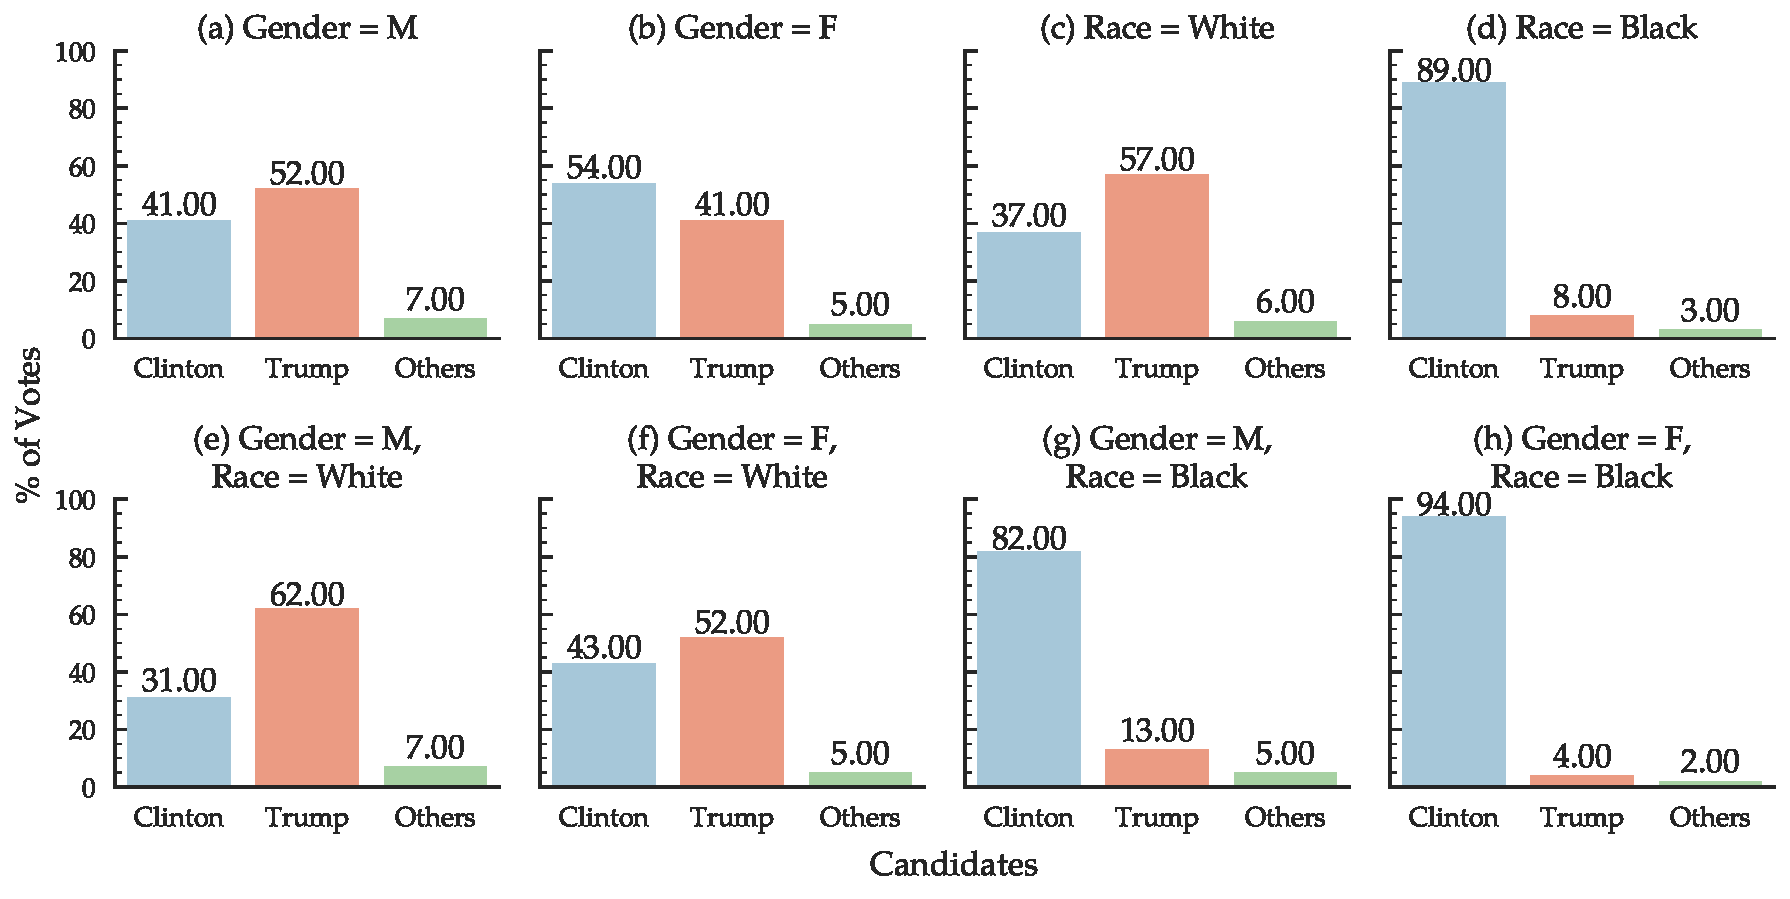
\includegraphics[width=\linewidth]{figures/US_Election_Example.pdf}
%   \caption{A set of visualizations from the 2016 Election polls. These visualizations show the percentage of votes for three candidates (Donald Trump, Hilary Clinton, and Others) in different demographic groups (based on race and gender).}
%   \label{fig:elections_example}
% \end{teaserfigure}


% \begin{figure*}[bht]
% \centering
% 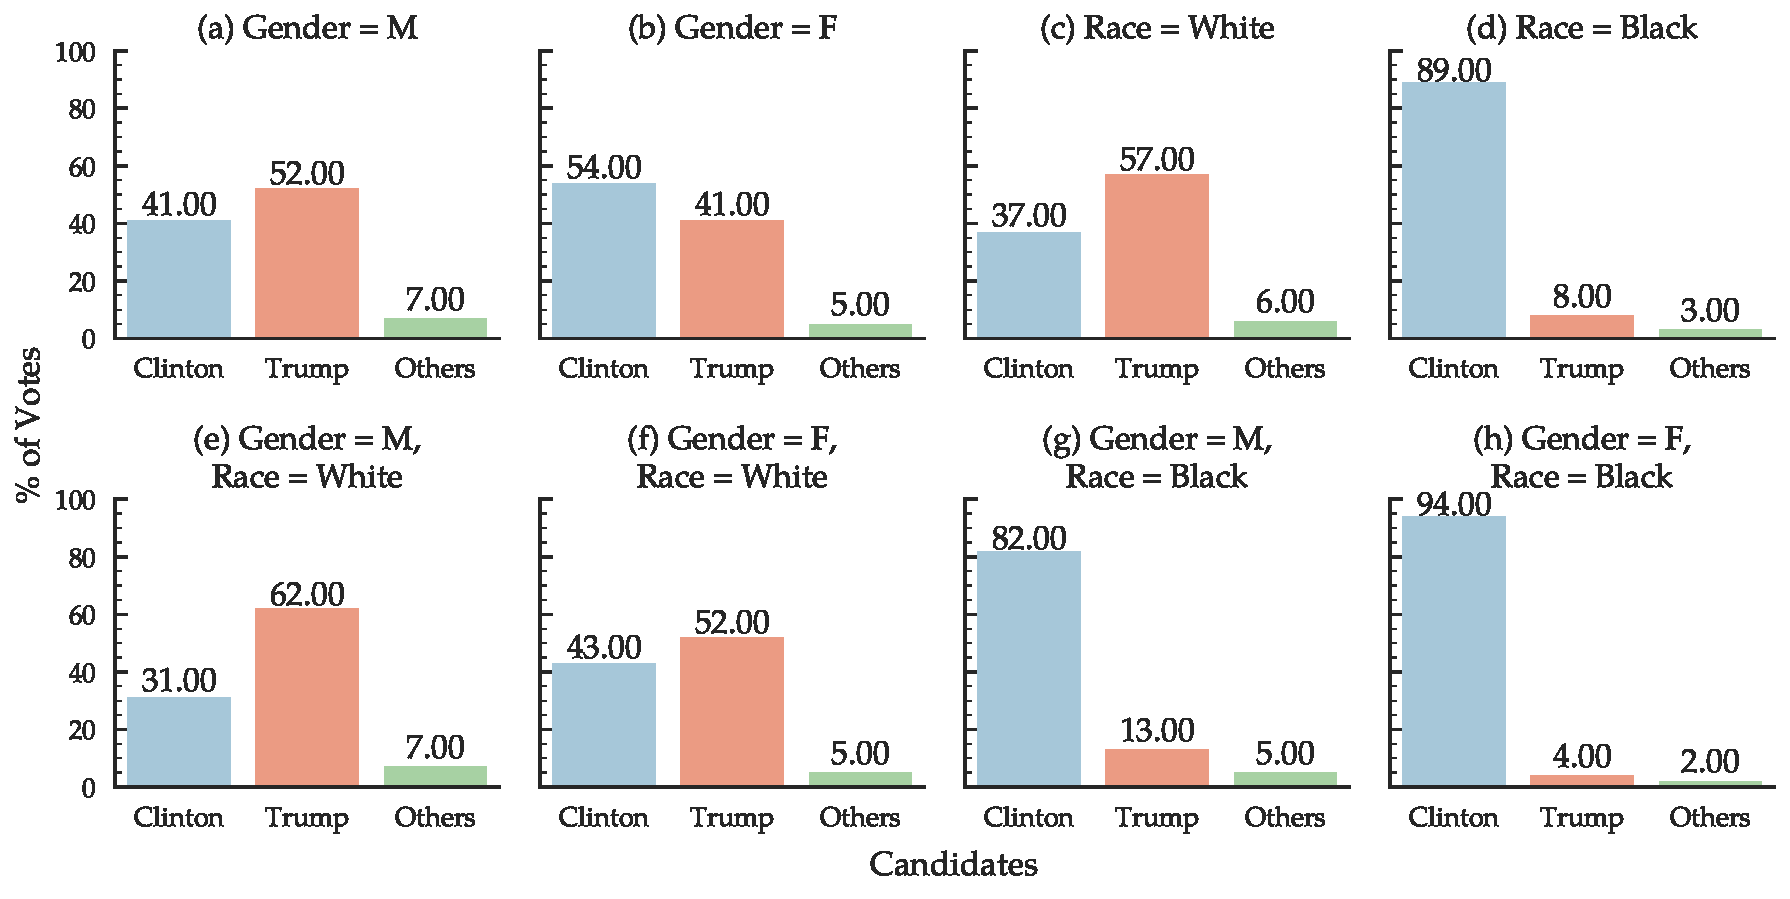
\includegraphics[width=\linewidth]{figures/US_Election_Example.pdf}
% \caption{A set of visualizations from the 2016 Election polls. These visualizations show the percentage of votes for three candidates (Donald Trump, Hilary Clinton, and Others) in different demographic groups (based on race and gender).}
% \label{fig:elections_example}
% \end{figure*}

\section{Introduction}

%\hdev{Let's take a step back, and look at the current flow in introduction. In the first paragraph, we vaguely motivate what can be considered as collective insights. In second paragraph, we try to connect the idea of collective insights with the challenges of data subset exploration. In third paragraph, we introduce two concepts: visual summarization, and distribution awareness. We do not clearly state what these two means. There's an example that conveys what could be captured through pattern or trend mining. In the fourth paragraph, we present an example to convey some specific challenges of visual summarization. The fifth paragraph states our contributions. My suggestion is to immediately jump into business by saying what we mean by distribution awareness, why is it important, and why is this challenging. We have the contents lying around already, it's just a matter of clearly stating these three aspects, preferably without using new abstractions.}

Common analytics tasks, such as causal inference, feature selection, and outlier detection requires studying the distributions or patterns at different granularities of data [Refs]. For example, a campaign manager may study the voting patterns in different demographics (based on race, gender, social class etc.) using the 2016 US election exit polls\footnote{\url{https://edition.cnn.com/election/2016/results/exit-polls}} to identify the nonconformist demographic groups. Visual analysis is the \emph{de facto} approach for performing such analytics tasks [Refs], where an analyst constructs visualizations to capture the distributions at different subsets of data. The goal of this visual analysis is to extract meaningful insights---when a set of visualizations along with human interpretation leads to informative and interesting facts arising from the distributions.

However, without knowing \textit{what} subset of data contains an interesting distribution, manually exploring all possible data subsets can be tedious and inefficient for an analyst. For example, the aforementioned campaign manager could construct bar charts for different demographics, where x-axis shows the election candidates and y-axis the percentage of votes for these candidates. Subsequently, he could compare these bar charts to understand how voting pattern changes across different demographics. Both of these exercises, first, constructing the large number of visualizations corresponding to all possible data subsets, and then, navigating through this large space of visualizations to draw meaningful insights is challenging. Currently, there is no systematic way to perform these exercises. 

To this end, we present \system, an interactive visualization summarization system that automatically selects a small set of visualizations to summarize the data distributions within a dataset in an informative manner. When analysts inspect informative visualizations that cover these insights, they associate particular sets of attributes to typical trends and observed patterns. We define this aspect of dataset understanding as \emph{distribution awareness}. For example, we observe that in Figure~\ref{fig:elections_example}, most of the visualizations has `Clinton' and `Trump' as comparably-sized bars with `Others' being a small fraction of the overall (a,b,c,e,f), whereas visualizations involving the Black population is highly skewed towards `Clinton' (d,g,h). Since human analysts have limited memory and attention, it is often impossible to visualize all possible data subsets. An ideal summarization system should display visualizations that enables users to gain maximal distribution awareness of the typical trends within a dataset. 

%Even after constructing the visualizations for all possible data subsets, which itself is a daunting task, currently there is no systematic way for our campaign manager to make sense of or even navigate through this large space of possible visualizations to draw meaningful insights. 

%\par The goal of visual analysis is to extract meaningful stories or insights from the data. Individual visualizations represent simple ``factoids'' portraying one aspect of the data. Meaningful insights arise when a group of factoids work in conjunction, along with human interpretation, to produce informative and interesting facts. 
%\par However, without knowing \textit{what} subset of the data would be interesting to visualize, manual drill-downs and roll-ups on all possible filter combinations can be tedious and inefficient for analysts. In many data analytics scenarios, analysts have an x and y axis of interest and want to explore data subsets corresponding to different filtering criteria. For example, a campaign manager may be interested in looking at bar chart visualizations of x as the voted candidate and y as the percentage of votes for the 2016 US elections exit polls with different filter combinations on demographics information, such as gender, income, race, states, and responses to different survey questions\footnote{\url{https://edition.cnn.com/election/2016/results/exit-polls}}. The analyst would have to compare across a combinatorially large space of different data subsets by iteratively changing the filter criterion of a visualization to understand how the relationship between the x and y variables change across data subsets. Even if the analyst had plotted visualizations for all possible data subsets, currently there is no systematic and effective way for an analyst to make sense of and navigate through the large space of possible visualizations to draw meaningful insights. 
%\par To this end, we present \system, an interactive visualization summarization system that automatically selects a small set of visualizations to summarize the data distributions within a dataset in an informative manner. When analysts inspect informative visualizations that cover these insights, they associate particular sets of attributes to typical trends and observed patterns. We define this aspect of dataset understanding as \emph{distribution awareness}. For example, we observe that in Figure~\ref{fig:elections_example}, most of the visualizations has `Clinton' and `Trump' as comparably-sized bars with `Others' being a small fraction of the overall (a,b,c,e,f), whereas visualizations involving the Black population is highly skewed towards `Clinton' (d,g,h). Since human analysts have limited memory and attention, it is often impossible to visualize all possible data subsets. An ideal summarization system should display visualizations that enables users to gain maximal distribution awareness of the typical trends within a dataset. 
%\par However, finding effective visualizations to summarize a dataset is not as trivial as picking individual visualizations that maximizes some statistical measure, such as deviation~\cite{Vartak2015}, coverage~\cite{Sarvghad2017}, or significance testing~\cite{Anand2015}, which can often result in misleading summarizations. Consider an elections campaign manager who is allocating the advertisement budget to be spent on different demographic populations to target for an upcoming election by investigating the voting patterns across different demographic groups. He performs a randomized permutation testing between the gender and race attributes and finds that the voting pattern of black females is drastically different from the voting pattern of general female population and allocates the his advertisement funds to target the black female population. \dor{Himel, can you check if this example makes sense? or should we say chi2? chi2 just give you columnar correlation info not at the attribute-level info? although probably only a deviation based comparison can give you a comparison like this.} While black females do defy the trends of general females, the comparison is incomplete, since it ignores the fact that black females follows very closely to the distribution of the voting behavior of the black population, so the proper subpopulation to target should be the black population rather than the more specific black female population.
%\par The above example showcases a scenario where the selection of an improper reference (female) for comparing the visualization (black female) against results in misleading insights. In \system, we formulate an objective where a visualization is \emph{actually} interesting when it deviates from and can not be explained by \emph{even} its most informative reference. \dor{can we add an example here?} Our user study results described in Section~\ref{sec:userstudy} shows that this notion of informative interestingness can guide an analyst towards more meaningful stories for further investigation. 
\par The contribution of this paper include: 
\begin{denselist}
\item Proposing the novel problem of visualization summarization and use cases highlighting the importance of \textit{distribution awareness} in dataset understanding (Section~\ref{sec:distributionaware}), %inform  visualization understanding and analytical tool designs
\item Formulating the structure and utility of the visualization search space (\emph{lattice}) using a user expectation model motivated by our formative study (Section~\ref{sec:datamodel}),
\item Designing efficient algorithms and optimizations to identify a set of informatively connected interesting visualizations (Section~\ref{sec:system}),  
\item Presenting an interactive visualization dashboard interface that adopts a simple and intuitive hierarchical lattice layout (Section~\ref{sec:interaction}),
\item Demonstrate the efficacy of our system through a user study evaluation (Section~\ref{sec:userstudy}).
\end{denselist}
%!TEX root = main.tex
% \section{Towards Informative Exploration}
\change{\section{Problem Formulation\label{sec:problem}}}
In this section, we first describe how analysts
manually explore the space of data subsets.
We then introduce \change{three design principles
for a system that can automatically guide analysts to the key insights}.
% \subsection{Manual Exploration via Drill-Downs}

\change{\subsection{Manual Exploration: Approach and Challenges}}
During visual data exploration,
an analyst may need to explore different subsets
of the data \change{that together form a combinatorial \emph{lattice}}.
Figure~\ref{fig:elections_example}
shows a partial lattice for the 2016 US election dataset.
The lattice contains the overall visualization
with no filter at the first level,
all visualizations with a single filter
at the second level \change{(such as \fem)},
all visualizations with two filters at third level,
and so on.
Analysts explore such a combinatorial lattice
from top to bottom, by generating and examining
visualizations with increasing levels of specificity.
In particular, analysts perform \emph{drill-downs}~\cite{Gray1997}
to access data subsets at lower levels by
adding one filter at a time
\change{(such as adding \blk to \fem along the purple path)}
and visualize
\change{their measures of interest for each data subset---in
this case the percentage of votes for each candidate}.
Further, as analysts perform drill-downs,
they use the most recent visualization
in the drill-down path---the {\em parent}---as a \change{{\em reference}}
to establish what they expect to see in the
\change{next visualization in the path---the {\em child}}.
In Figure~\ref{fig:elections_example},
the visualizations \fem and \blk
are the \emph{parents} of the \blkfem visualization,
explored along the purple and orange path respectively.

\par \change{As we saw in the purple path
in Figure~\ref{fig:elections_example},
while performing drill-downs,
analysts may detect a local deviation
(we will formalize these and other notions subsequently)
between
a parent and a child to be significant.
For example, they may be surprised by the fact
that the \fem and \blkfem
visualizations are very different from each other,
and may
find this to be a novel insight.
However, this deviation is a result of \fem
not being an
{\em informative}
parent or reference for \blkfem---instead, it is a
{\em deceptive} reference.
Here, a different parent, \blk,
is the most informative parent or reference of \blkfem
because it is the parent that exhibits the
least deviation relative
to \blkfem.
Here, the \blkfem visualization
is not really all that surprising given the \blk
visualization.
We refer to this phenomenon of being deceived by
a local difference or deviation relative to a deceptive
reference as an instance of the {\em drill-down fallacy}.
One way to avoid such fallacies is to ensure that one or more
informative parents
are present for each visualization so that analysts
can contextualize the visualization accurately.
While this fallacy is applicable to any
chart type that can be described as a
probability distribution over data
(e.g., pie charts, heatmaps),
we will limit our discussion to bar charts for brevity.}

% \subsection{Three Elements of Informative Exploration}
\change{\subsection{The ``3S'' Design Principles}}
Our goal is to help analysts discover
the key insights in a dataset while avoiding drill-down fallacies.
We \change{outline}
three essential principles for
finding such insights---the three S's:
\emph{safety}, \emph{saliency}, and \change{\emph{succinctness},
and progressively layer these principles to formalize
a measure of utility for a network of visualizations}.
We adopt these principles to
develop a visual exploration tool
that \change{automatically generates
a network of visualizations conveying the key
insights in a multidimensional dataset}.

\subsubsection{Safety}
\change{To prevent
drill-down fallacies,
we ensure {\em safety}---by making sure
that informative parents are present
to accurately contextualize visualizations.
A parent is said to be {\em informative}
if its data distribution closely follows the child
visualization's data distribution,
since the presence of the parent allows
the analyst to form an accurate mental model
of what to expect from the child visualization.
We compute the informativeness of
the $j^{th}$ parent $V_i^j$
for a visualization $V_i$
as the similarity between their data distributions
measured using a distance function $D$.
For bar charts, the data distribution refers to
the height of bars assigned to the categories labeled by the x-axis,
suitably normalized.
Accordingly, the computed distance
$D(V_i, V_i^j)$
refers to the sum of the distances
between the normalized heights of bars across different categories.
Quantifying deviation using distances between normalized versions of visualizations
in this manner is not a novel idea---we leverage prior work for this~\cite{Vartak2015,Siddiqui2017,Macke2018,Ding2016}.
The specific distance measure $D$ is not important; while we use the Euclidean metric,
we can easily work with other common distance metrics such as Kullback-Leibler Divergence and Earth Mover's distance~\cite{Vartak2015}.
The most informative parent $V_i^\dagger$ for a visualization $V_i$ is
the one whose data distribution is most similar to $V_i$.
}
%The distance $D(V_i, V_i^j)$ is computed based on the probability distributions represented by each visualization (in this case, a vector of bar values). \tr{For example, based on the Figure~\ref{fig:elections_example} example, the Euclidean distance between \fem ($V_i^j$=[54,41,5]) and \blkfem ($V_i$=[94,4,2]) is 54.57.} sqrt((94-54)**2+(41-4)**2+3**2)

\begin{equation}
    V_i^\dagger= \underset{V_i^j}{argmin}\ D(V_i, V_i^j)
\end{equation}
\change{Instead of insisting that the most informative
parent is always present to contextualize a given child visualization,
we relax our requirement somewhat: we don't need {\em the
most} informative parent to be present, just {\em an} informative parent.
We define a parent to be informative (denoted $V_i^*$) if its distance from the child falls within a threshold $\theta\%$ of the
most informative parent---the default is set to 90\%
and adjustable by the user.}
\cut{
    We regard a parent visualization as informative if its distance from the child visualization falls within a threshold $\theta\%$ compared to the most informative parent:
    \begin{equation}
        V_i^{*, \theta} = \{V_i^j : \frac{D(V_i, V_i^*)}{D(V_i, V_i^j)} \geq \theta\}
    \end{equation}
    For example in Figure~\ref{fig:elections_example}, while both \blk and \fem visualizations are considered parents of the \blkfem visualization, only the \blk visualization is considered an informative parent of the \blkfem population, for any values of $\theta \geq 11\%$ via the Euclidean distance metric.
}
\subsubsection{Saliency}
\change{Simply ensuring that
informative parents are present is insufficient;
we also want to emphasize {\em saliency} by
identifying visualizations that convey new information.
In general, a visualization is deemed to be \emph{interesting}
if its underlying data distribution differs
from that of its parents,
and thus offers new unexpected information or insight.
Such distance-based notions of interestingness
have been explored in past work~\cite{Correll2016,Itti2009,Vartak2015},
where a large distance from some reference visualization
indicates that the selected visualization is interesting.
We deviate from this prior work in two ways:
first, we concentrate on {\em informative} interestingness,
where the interestingness of a child visualization
is only defined with respect to informative parent references.
Second, we weigh the interestingness by the proportion of the
population captured by the child visualization.
(That is, when a deviation is manifested in a larger population,
it is deemed to be more significant and therefore more interesting.)
Thus, we define the utility of a visualization $V_i$, $U(V_i)$ as follows:
 $$
    U(V_i)=
\begin{cases}
     \frac{|V_i|}{|V_i^*|} \cdot D(V_i, V_i^*) & \text{if } V_i^* \text{ is present}\\
    -\infty             & \text{otherwise}
\end{cases}
$$
That is, the utility or interestingness of a visualization
is the distance between the visualization and its informative
parent, if present\footnote{If multiple informative parents, $V_i^*$, are present for a given visualization, $V_i$, then $U(V_i)$ is defined in terms of the most informative parent present.}. To incorporate the effect of subpopulation size into our objective function, we multiply the distance $D(V_i, V_i^*)$ between an informative parent $V_i^*$ and a child visualization $V_i$ by the ratio of their sizes.
Notice that the objective $U$ has a minimax form~\cite{wiki:minimax},
in that informativeness aims to minimize the distance between parent and child,
while interestingness aims to maximize the resulting minimum distance.
For convenience, we define $U(V_0)$, where $V_0$ is the overall visualization,
to be $1$, which is the maximum value that the expression $\frac{|V_i|}{|V_i^*|} \cdot D(V_i, V_i^*)$ can take, ensuring that the overall visualization
is always valuable to include.
}

\subsubsection{Succinctness}
\change{
We cannot possibly display all of the visualizations
in the lattice of data subsets: this lattice scales
exponentially in the number of attributes.
Instead, we aim for {\em succinctness},
where we only select a subset $S$ of size $|S| = k$ from all the visualizations.
We define the utility of $S$ as follows:
$$U(S) = \sum_{V_i \in S}{U(V_i)}$$
In this subset, for every visualization except for the overall
visualization, one of its informative
parents must be present (otherwise $U = -\infty$).
Thus, this subset ends up being a connected network
(a sub-graph of the overall lattice) rooted at the overall visualization,
ensuring that for each visualization, there is an informative parent available
for context.
We can now formally define our problem statement.
\par \textsc{Problem.} \textit{Given a dataset and user-provided X, Y attributes,
select a subset $S$ of $|S| = k$ visualizations from the lattice of data
subsets $\mathcal{L}$, such that $U(S)$ is maximized.}
\\
Thanks to how we have defined $U$, $S$ will include the overall visualization,
corresponding to the entire dataset with no filter. And,
for each visualization in $S$ except the overall one,
at least one of its informative parents will be present in $S$.
This network of visualizations $S$ can be displayed on a dashboard.
}
% To succinctly convey insights, we concentrate on \emph{summarization}---identifying a group of visualizations that collectively contain informative insights. Since our aim is to identify a unified narrative, instead of discrete insights, we enforce that any selected visualization must have at least one of its informative parents present in the dashboard. Specifically, we identify a set of $k$ connected visualizations that collectively maximize the sum of the proposed utility $U(V_i)$ across each selected visualization, $V_i$, and thus succinctly convey informative insights, more formally stated as follows:
% \par \textsc{Problem.} \textit{Given a dataset and user-provided X, Y attributes, select $k$ visualizations from the lattice of data subsets $\mathcal{L}$ to be included in the dashboard, such that:
% \\ (i) one of the selected visualization is the overall visualization, corresponding to the entire dataset with no filter;
% \\ (ii) for each visualization except for the overall, at least one of its informative parents is present in the $k$ visualizations;
% \\ (iii) the $k$ selected visualizations maximize the total utility $\sum_{V_i \in \mathcal{L}} U(V_i)$ as defined above.
% }
% and aggregation function G, a lattice $\mathcal{L}$ consisting of visualizations $V_i$ for all possible filter $F_i$ that could be constructed from dataset D:}
% \\ \texttt{$V_i$ = SELECT X, G(Y) FROM D WHERE $F_i$ GROUP BY X}
% \\ \textit{find k visualizations from $\mathcal{L}$ to include in dashboard $\mathcal{S}$, such that the total utility $\sum_{V_i \in \mathcal{L}} U(V_i)$ as defined above is maximized, while enforcing that all $V_i \in \mathcal{S}$ is connected.}
\change{Since the edges between non-informative parents to children are not pertinent to the solution, we can remove those edges from the lattice, leaving only the edges from the informative parents to the children. Then, we are left with an arbitrary graph, from which we need to select a rooted subgraph of size $k$, with greatest utility $U$.}
\par \tr{For arbitrary distance metrics $D$, we can show that our problem is {\sc NP-Hard} via a reduction from the AND-graph prerequisite problem, which has been shown to be {\sc NP-Hard} in ~\cite{Parameswaran2010}. Similar to our problem, in the AND-graph prerequisite problem, all prerequisites need to be taken before a node can be selected. Both the scoring function in the prerequisite problem and the distance-based utility in our problem are non-negative and independent of selection order. Furthermore, both the AND-graph in the prerequisite problem and our lattice have only directed edges across neighboring levels (i.e. only edge connections from n$\rightarrow$n+1). Based on our informativeness criteria, some directed edges may not be present in the graph. These pruned edges are equivalent to the AND-graph case where the score is zero. For a distance metric D, two nodes are discernable if the distance between them is zero. Hence, we prove by bijection that the two problems are equivalent and thereby proving that our problem is NP-hard.}
% Unfortunately, the problem of finding a
% connected subgraph in a lattice with
% maximum total edge utility is known
% as the \emph{maximum-weight connected subgraph problem}~\cite{ErnstAlthaus2009}
% and is known to be {\sc NP-Complete}~\cite{Parameswaran2010}.
% \agp{This doesn't actually show that our problem is hard. We need to reduce max-weighted subgraph to our problem, not the other way around. I am leaving a pointer here to think about it later.}
\change{Next, we design an approximate algorithm
 to solve this problem.}

%!TEX root = main.tex
\begin{figure}[h!]
\centering
\vspace{-10pt}
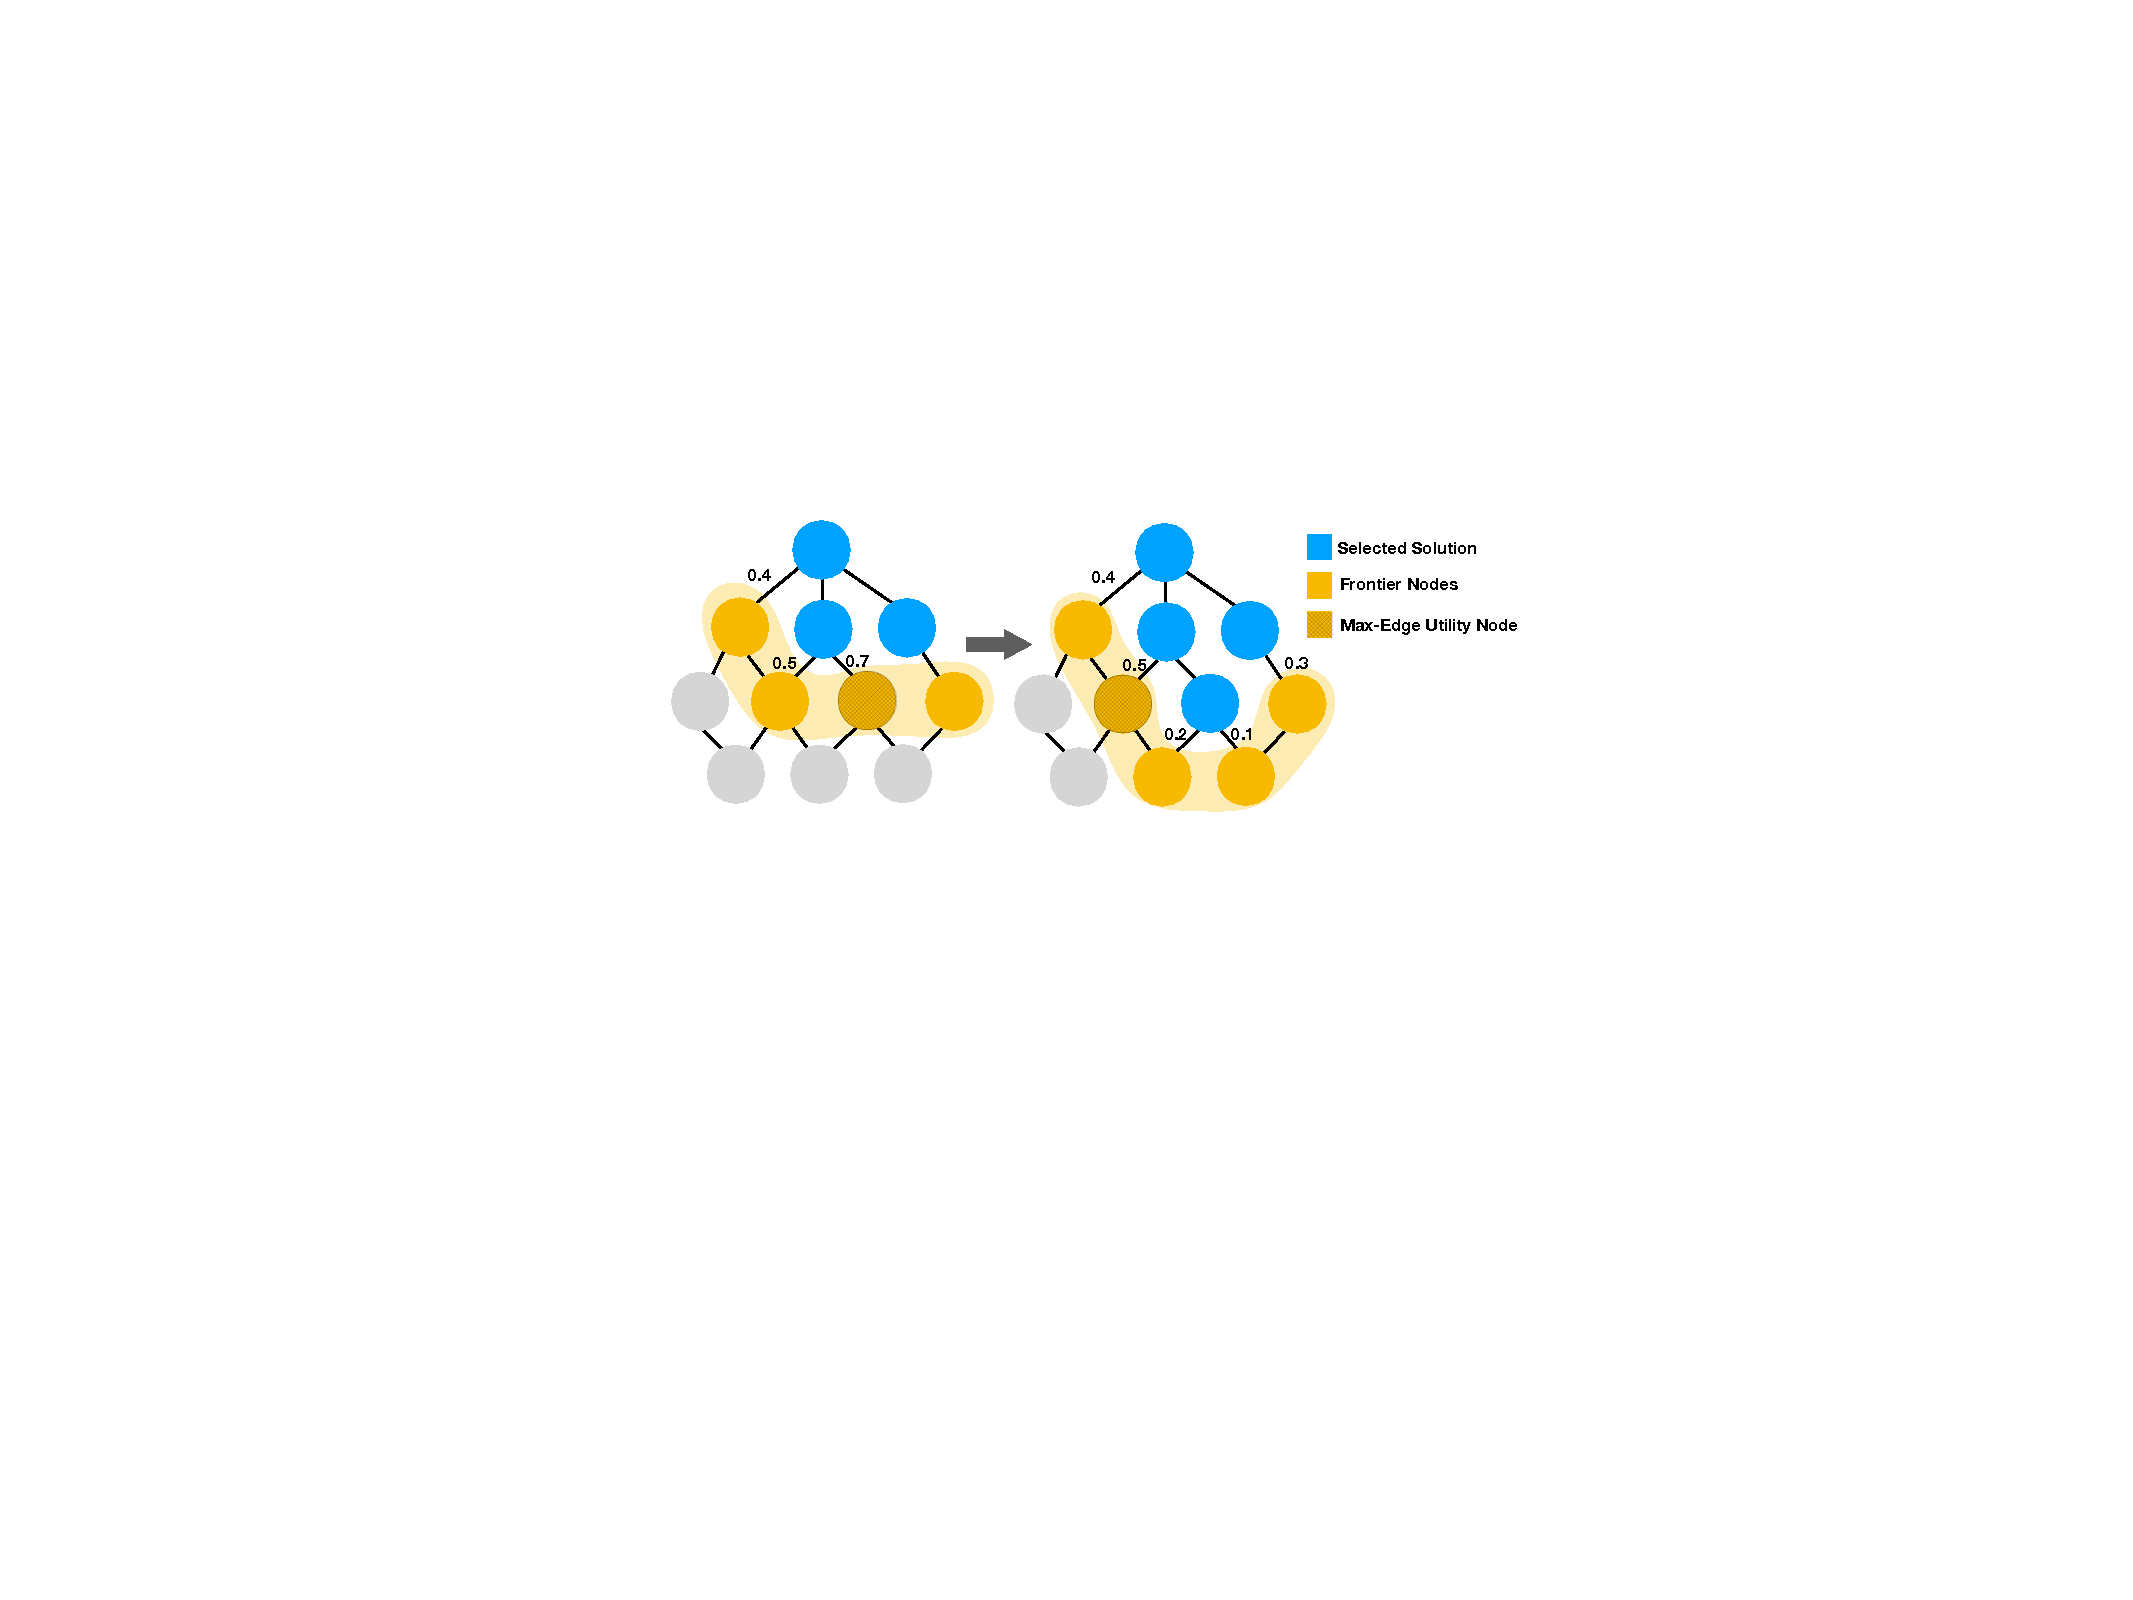
\includegraphics[width=\linewidth]{figures/frontier_greedy.pdf}
\vspace{-20pt}
\caption{Example illustrating how the frontier greedy algorithm incrementally builds up the solution by selecting the maximal-edge utility node from the frontier at every step. \achange{Starting from a pre-materialized lattice consisting of only connections to informative parents (left) and three nodes in the existing} solution (blue), we select the node with the highest edge utility \change{(yellow)} amongst the frontier nodes \change{(green)}. On the right, the newly added node results in an updated frontier and a maximum-edge utility node is selected amongst them.
\agp{I think the edge weights in the figure are really confusing. I would propose dropping it. Or, attach the utility to the nodes instead of the edges. In this case, I would say it might be interesting to set the utility of the 0.5 node to be $-\infty$ until the one with 0.4 is added first (an informative parent, perhaps). That will add to the richness of the example. Right now I can't tell if the example has edge-weights, node-weights... overall, I can't even tell what the mapping to the utility is here.}\dor{Changed.}
}
\vspace{-10pt}
\label{fig:frontier_greedy}
\end{figure}
\section{Storyboard System\label{sec:system}}
In this section, we present our system, \system, by first providing a high-level overview of the underlying algorithms, and then describing the user interaction mechanisms.
\change{
  \subsection{Lattice Traversal Algorithm\label{sec:algorithms}}
  \achange{For a given dataset and user-selected X, Ys, we first enumerating all possible attribute-value combinations (i.e. filters) to construct the lattice by  retaining only edge connections to informative parents. Now, we }discuss the algorithm used for traversing the
  lattice to select the connected subgraph $S$ of $k$
  visualizations (or equivalently, nodes in the lattice) that maximize
  the utility $U$.
}%generating the visualization lattice, and then present an overview of how we
\tr{
\stitle{Lattice Generation:} Our system supports two variants of traversal based on the lattice generation procedure---offline variants that first generate the complete lattice and then work towards identifying the solution with maximum combined-edge utility, and online variants that incrementally generate the lattice and simultaneously identify the solution. The offline variants are appropriate for datasets with a small number of low-cardinality attributes, where we can generate the entire lattice in a reasonable time; whereas the online variants are appropriate for datasets with many high-cardinality attributes, where we need to incrementally generate a partial lattice. \tr{
  To prevent the danger of visualizations with small population size, users can also select an \textit{iceberg condition} ($\delta$) to adjust the extent of pruning on visualizations whose sizes fall below a certain percentage of the overall population size. \footnote{The terminology is used in the discussion of iceberg cubes in OLAP literature~\cite{Xin2007}.}
}
%In most cases, the lattice contains a large number of visualizations due to the presence of many attributes or high-cardinality attributes in the dataset. In such cases finding an optimal solution is computationally challenging.
\stitle{Lattice Traversal:} We first describe the offline version of the algorithm before outlining the modification required for the online variant of the algorithm. Given a lattice that has been materialized offline,
}
\change{Our algorithm,
titled {\em frontier-greedy}, is inspired
\achange{by the notion of ``externals'' in Parameswaran et al.}\cite{Parameswaran2010}.
The algorithm incrementally grows a subgraph $S'$ until
$k$ nodes are selected.
Throughout, the algorithm maintains a \achange{set} of {\em frontier} nodes \achange{$\mathcal{F}$}---nodes
that are connected to the existing subgraph solution $S'$
but have not yet been
added. The frontier nodes includes all of the children of the nodes
in $S'$. \achange{Given that our pre-materialized lattice only contain edge connections to informative parents, any frontier node is guaranteed to have an informative parent in the the existing solution and can be added to $S$ without violating the informativeness principle.}
%Any frontier node whose informative parent is present in the existing solution can potentially be added to the existing solution, without violating the informativeness principle.
At each iteration, the algorithm adds the node from the frontier
nodes that leads to the greatest increase in the utility of $S'$: i.e.,
the node $V_n$ such that $U(S' \cup \{V_n\})$ is the largest.
Figure~\ref{fig:frontier_greedy} displays how the algorithm
maintains the list of frontier nodes (in green), and the current $S'$ (in blue),
adding the node that leads to the greatest increase in utility (in yellow).
Algorithm~\ref{algo:frontier_greedy} provides the pseudocode.
}
\begin{algorithm}
  \begin{algorithmic}[1]
  \Procedure{PickVisualizations}{$k$, \achange{$\mathcal{L}$}}
  \State $S' \gets$ \{$V_0$\}  \text{/* adding the overall node */}
  \While{$|S'| < k$}
      \State \achange{$\mathcal{F}$} $\gets$ getFrontier($S'$, \achange{$\mathcal{L}$})
      \State bestUtility $\gets$ $U(S')$
      \For{$\achange{V_i}$ $\in$ \achange{$\mathcal{F}$}}
      \If{$U(S' \cup \{\achange{V_i}\})>$bestUtility}
      \State maxNode $\gets$ $\achange{V_i}$
      \State bestUtility $\gets U(S' \cup \{\achange{V_i}\})$
      \EndIf
      \EndFor
      \State $S' \gets S' \cup$ \{maxNode\}
  \EndWhile
  \Return $S'$
  \EndProcedure
  \end{algorithmic}
  \caption{Frontier Greedy Algorithm\agp{The pseudocode had some inaccuracies that I tried fixing. Please carefully check.}\dor{Minor changes. Do we need to initialize maxNode in the pseudocode? For bestUtility $\gets U(S')$, would it be more clear if we initialize as bestUtility $\gets -\infty$?}}\label{algo:frontier_greedy}
\end{algorithm}
%The frontier greedy algorithm first compiles a list of candidate nodes known as the \textit{frontier} nodes, which encompasses all nodes that are connected to the existing subgraph solution. As long as the informative parents of frontier nodes are already present in the solution, the frontier nodes can be appended to the current solution without violating requirement (ii) in the problem formulation, enforcing the presence of informative parent for every selected visualization. To obtain the frontier nodes, the algorithm scans and adds all children of leaf nodes of the current dashboard as part of the frontier. \tr{In the online version, it additionally checks for each child whether its informative parent is present in the current dashboard.} As illustrated in Figure~\ref{fig:frontier_greedy}, at each step, our algorithm greedily picks the node with the maximum edge utility amongst the eligible frontier nodes to add to the current solution, and updates the frontier accordingly. \ccut{The \textit{frontier greedy} algorithm discussed here is used for generating the dashboards for our user study and we defer the details of other algorithms that we have developed for lattice traversal to the technical report. }
%\par The frontier greedy algorithm obtains a list of candidate nodes known as the \textit{frontier} nodes, which encompasses all neighbors of nodes in the existing subgraph solution. Any of the nodes in the frontier can be added to the current solution since their informative parent is present in the solution. To obtain the frontier nodes, the algorithm scans and adds all children of leaf nodes of the current dashboard as part of the frontier. In the online version, it additionally checks for each child whether its informative parent is present in the current dashboard. At each step, our algorithm greedily picks the node with the maximum utility amongst the frontier nodes to add to the current solution, and updates the frontier accordingly. \tr{The path merging algorithm first generate the informative paths from root to every candidate node. Then, it greedily merges the paths with high-utility to create a subgraph whose size is less than or equal to maximum capacity $k$.}

\subsection{User Interaction\label{sec:interaction}}
\begin{figure*}[ht!]
\centering
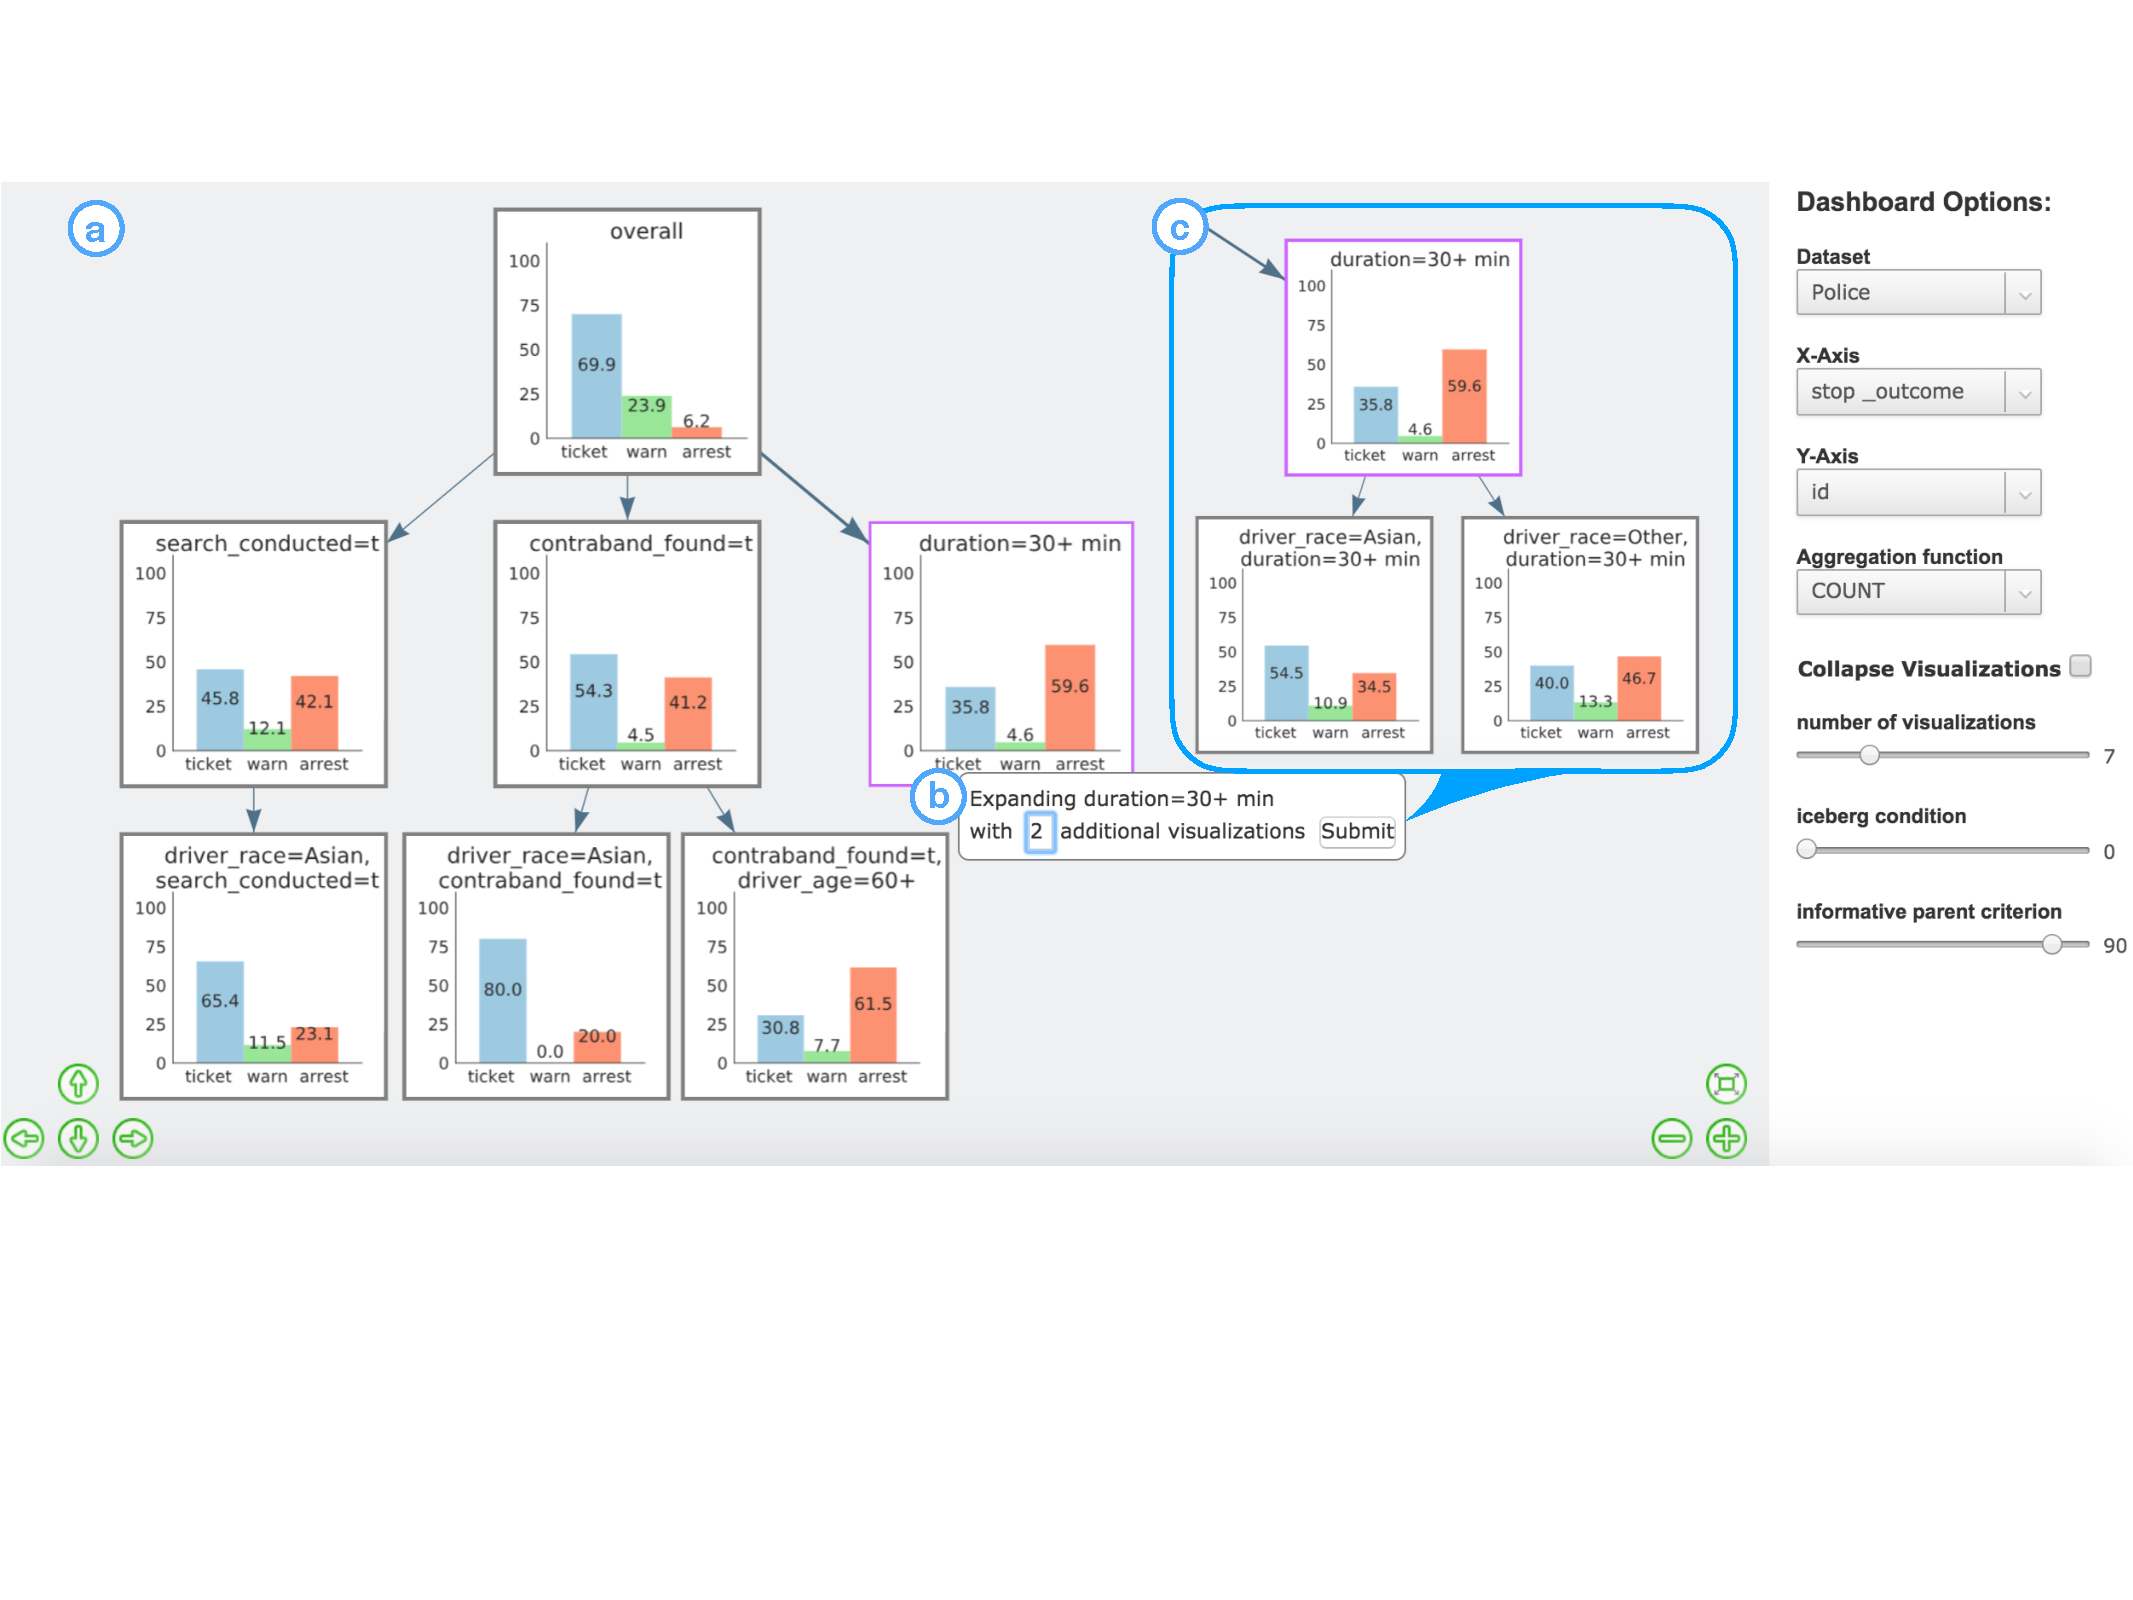
\includegraphics[width=0.9\linewidth,frame]{figures/overview_interface_expand.pdf}
\caption{a) Overview of the \system interface for the Police Stop dataset. Users can  select \change{x, y axes, and aggregation function via the dropdown menu, to define the visualization space of interest, as well as adjusting dashboard parameters, such as the number of visualizations to show in the dashboard (k) via the sliders.} b) User clicks on the duration=30+min visualization to request 2 additional visualizations. c) A preview of the added portion of the resulting dashboard is shown.}
% Default values are set for system related parameters such as the number of visualizations to show in the dashboard (k), iceberg condition for pruning ($\delta$), and informative parent criterion ($\theta$), which can be adjusted by the users via the sliders if needed.
\label{fig:overview}
\vspace{-10pt}
\end{figure*}%optional system parameter settings

\change{Given the visualizations in $S'$,
we can render these visualizations in a dashboard,}
where users can inspect the \change{visualizations}
through panning and zooming with navigation buttons,
mouse clicks, and key bindings.
Users can also select the x and y axes of interest,
aggregation function, and \change{set the number of visualizations ($k$)}
to generate a dashboard.
\change{Figure~\ref{fig:overview} displays
\system in action on the Police stop dataset~\cite{police}.
}
The dataset contains records of vehicle and pedestrian stops from law enforcement departments in Connecticut, dated from 2013 to 2015. In this case, the analyst is interested in the percentages of police stops \change{(Y)} that led to different outcomes \change{(X)}, such as ticket, warning, or arrest.
\change{As shown in Figure \ref{fig:overview}a, the analyst
may begin by generating a 7-visualization dashboard.
\achange{She} would learn that if a search is conducted (\texttt{search\_conducted=t}),
then the probability of being arrested increases from \achange{6.2\% to 42.1\%}.
However, the probability goes down to \achange{23.1\%}
if the driver is Asian (\texttt{driver\_race=Asian, search\_conducted=t}).
When examining these visualizations, the analyst can be confident that
any deviations are both informative and interesting: that is, the informative
parents are present for each child,
making the takeaways more significant.
Moreover,
the analyst may learn that for drivers
who had contraband found in the vehicle (\texttt{contraband\_found=t}),
the arrest rate for those who are 60
and over is surprisingly higher than usual,
whereas for Asian drivers the arrest rate is lower.
}

After browsing through visualizations in the dashboard,
\achange{the analyst} may be interested in getting more information
about a specific visualization.
\system allows \achange{analysts} \change{to perform additional
drill-downs by requesting}
a new dashboard centered on a chosen visualization
of interest as the new starting point
(or equivalently, the root of the lattice)
for analysis.
Say the analyst is now interested in learning more
about the other factor that contributes to \achange{high arrest rates}:
\change{a long stop with \texttt{duration=30+min}}.
In Figure~\ref{fig:overview}b, \achange{she}
can click on the corresponding visualization
\change{to} request additional visualizations.
Upon seeing the updated dashboard in Figure~\ref{fig:overview}c,
she learns that any visualization
that involves the \change{\texttt{duration=30+min}}
filter is likely to result in high ticketing and arrest rates.
This implies that if a police stop lasts more than 30 minutes,
the outcome would more or less be the same,
independent of other factors such as the driver's race or age.
To generate the expanded dashboard, \system uses the same models
and algorithms as before,
except the \achange{the overall visualization $V_0$ at the root node is now set as the selected visualization}.
This node expansion capability is motivated
by the idea of \textit{iterative view refinement}
\change{common in other} visual analytics systems,
which is essential for users to iterate on and
explore different hypotheses~\cite{Hoque2017,Wongsuphasawat2016}.

%!TEX root = main.tex
\section{User Study Evaluation\label{sec:userstudy}}
\subsection{Methods}
We evaluate the utility of our tool by performing a user study focusing on addressing the research questions:
\begin{denselist}
	\item RQ1: How effective is our tool at discovering visualizations of interest?
	\item RQ2: How effective is our tool at helping user evaluate the importance of attributes within a given dataset?
	\item RQ3: How effective is our tool at guiding users towards safe and informative visualization references? 
	% in providing analysts with task-specific insights? (including identifying important features for prediction tasks and estimating the distribution of an unseen visualization)
	% \item RQ3: How useful are the visualizations in the recommended dashboard to analysts?
\end{denselist}

We recruited 18 participants with prior experience working with data. Participants include undergraduate and graduate students, researchers, and data scientists, with 1 to 14 years of data analysis experience (average = 5.61).  %This can include, but are not limited to, browsing and reading data, data cleaning and wrangling, data visualization and model building. The inclusion criteria is assessed based on a self-reporting basis in the pre-study survey.
%an average of 5.61 years of experience working with data.
There were 8 female participants and 10 male participants. No participants reported prior experience in working with the two datasets used in the study. In this between-group study, participants are randomly assigned two of the three dashboards with k=10 visualizations generated by following conditions. 
\stitle{\system:} The dashboards for this condition is generated by the frontier greedy algorithm (described in Section \ref{sec:algorithms}) and displayed in a hierarchical layout (as seen in Figure~\ref{fig:overview}). In order to establish a fair comparison with the two other conditions, we deactivated the interactive node expansion and dashboard navigation functionalities described in Section \ref{sec:interaction}, especially since the k=10 dashboard was small enough to function without the navigation tools.
\stitle{\BFS:} Starting from the overall visualization, $k$ visualizations is selected in level-wise order: sequentially adding visualizations at the first level with 1-filter combination one at a time, proceeding with the 2-, 3-, etc. filter combinations, until $k$ visualizations have been added to the dashboard. This baseline is designed to simulate the dashboard generated by a meticulous analyst who exhaustively inspects all possible visualization combinations. The chosen visualizations are displayed in a 5x2 table layout in the traversed order.
\stitle{\cluster:} K-Means clustering is performed on the dataset with $k$ clusters, corresponding to $k$, the number of visualizations to be shown in the dashboard. For each representative cluster, we select the visualization that has the least number of filter conditions for interpretability\footnote{Due to this requirement, the overall visualization is guaranteed to be picked as one of the displayed visualizations.} and display them in a 5x2 table layout. This baseline is designed to showcase a diverse set of pattern distributions within the dataset.

\par We randomize the ordering for each task combination to prevent confounding learning effects. The study begins with a 5 minute tutorial using dashboards generated from the Titanic dataset~\cite{titanic}. To prevent bias across conditions, participants were not provided an explanation of how the dashboard is generated and why the visualizations were arranged in a particular way. Then, participants proceeded onto the Police dataset~\cite{police} %, which contains visualizations of the \% of police stop that resulted in a warning, ticket, or an arrest.
, which contains a total of 312948 records of vehicle and pedestrian stops from law enforcement departments in Connecticut, dated from 2013 to 2015. We generate a dashboard of visualizations with bar charts with x-axis as the stop outcome (whether the police stop resulted in a ticket, warning, or arrest) and y-axis as the percentage of police stops that led to this outcome. The attributes in the dataset include driver gender, age, race, and the stop time of day, whether a search was conducted, and whether contraband was found.
\par Participants were given some time to read through a worksheet containing descriptions of the data attributes. Then, they were given an attention check question where they are given a verbal description of the visualization filter and asked about the distributions for the corresponding visualization in the dashboard. After understanding the dataset and chart schema, participants were asked to accomplish the following tasks in the prescribed order below:
\stitle{Retrieval:} Participants were asked to talk aloud as they interpret the visualizations in the dashboard and mark each visualization as either interesting, not interesting, or leave it as unselected. This task was intended to measure how well participants are at retrieving interesting visualizations (RQ1).

\stitle{Attribute Ranking:} Participants were given a worksheet with all the attributes listed and asked to rank the attributes in order of importance in contributing to a particular outcome (e.g. factors leading to arrest or autism diagnosis). Attribute ranking tasks are common in feature selection and other data science tasks. The goal of this task is to measure how well participants understand the relative importance of each attribute in contributing towards an outcome (RQ2).

\stitle{Shallow Prediction:} Participants were given a separate worksheet and asked to draw an estimate for a visualization that is not present in the dashboard. The visualization to be estimated is considered ``shallow'' if it is a visualization with 2 filter combinations, with one parent present in the given dashboard. After making the prediction, participants are shown the actual data distribution and asked to rate on a Likert scale of 10 how surprising the result was.

\stitle{Deep Prediction:} This task is similar to the shallow prediction, except that the visualization to be estimated is ``deep'' in the sense that it has 3 filter combinations, with only one parent in the given dashboard. Both prediction tasks measure how accurate the participants are at predicting an unseen visualization (RQ3).

\par The second dataset in the study is the Autism dataset~\cite{autism}, which includes the result of autism spectrum disorder screening for 704 adults. The attributes in the dataset are  binary responses to 10 diagnostic questions that are part of the screening process. Participants are not given the descriptions of the questions nor the answers corresponding to the labels. We generate dashboard visualizations based on whether the participant is diagnosed with autism or not. We repeat the same study procedure described above for the Autism dataset. At the end of the study, we asked two open-ended questions regarding the stories and insights that they have learned and what they like or dislike about each dashboard.
%The user study is composed of two phases. Phase one of the experiment focuses on comparing our tool against a set of baselines intended to simulate the natural sequence of visualizations that an analyst would encounter through various approaches during exploratory analysis. The baselines include:
%To prevent learning effects, the ordering of the baselines will be randomized across users.
% \par At the beginning of the study, participants were provided with a dashboard from an example dataset, as well as an explanation of how the dashboard is generated. For each of the visualization dashboard, participants are asked to mark visualizations as interesting/not interesting while explaining their reasoning for each annotation. Then, they are asked to summarize a list of insights that they have discovered after browsing through all visualizations in the dashboard. Participants also answer a set of task-specific questions related to causality and outliers[?], in the form as shown in the example [*]. These tasks are repeated for all baselines and our tool in randomized order on different datasets to prevent learning effects. At the end of phase one, participants are asked to comment on their experiences with each method, as well as the pros and cons of each of the tools. This phase of the experiment is designed to quantify the effects of RQ 1 and 2. In the end, we ask participants to discuss the interesting insights drawn from looking at the recommended dashboards as well as  ------.
%\par To prevent fatigue, after a 5 minute break, the participants then proceed onto phase two of the study, where they are given [10] dashboards generated by our tool and are asked to engage in a talk-aloud exercise as they browse the recommended visualizations. This is a more open-ended study intended for addressing RQ3 that can reveal our tool show unimportant results across different datasets and/or highlight larger selection of the types of insights that can be generated from the tool.
\subsection{Quantitative Results}
% In order to evaluate the efficacy of our system against the two baselines, we will first examine the quantitative results to address RQ1 and RQ2 and then discuss the qualitative findings to address RQ3.
%\dor{In general, we might have to make better connection between the RQs and the study results.}
\stitle{Retrieval (RQ1):} Using the click-stream data logged from the user study, we record whether each user is interested, not interested, or have not selected a visualization in the dashboard. %Since we do not have objective ground truths of which visualization is interesting or not, we use the participant's consensus to come up with a score for each visualization. In this scoring scheme, if visualization is marked as interesting, that visualization receives a score of 1; if a visualization is marked as uninteresting, the visualization incurs a penalty of -0.5\footnote{The reason why we chose a lower penalty score for disinterested clicks than the interested click reward is that some of the participants did not chose to mark visualizations that they thought were uninteresting as disinterested explicitly and chose to simply keep them unselected.}; no score is assigned if the visualization is unselected, then the scores are summed over all users who have seen the visualization. Each user is then assigned a score based on the product of their retrieval score and the consensus score (i.e. user would receive a higher score if selected visualization was highly ranked by consensus).
Since we do not have a objective ground truth on which visualization is interesting or not interesting, we devise a voting-based measure that measures how interesting is a visualization amongst all participants. As shown in Equation~\ref{weighting}, we assign a vote $\delta_{ij}$ of 1 if a user is interested in a visualization, 0 if they leave it unselected, and -1 if they are not interested in a visualization. Here i indexes the visualization and j indexes the user. 
\begin{equation}\label{weighting}
	\delta_{ij}= \left\{\begin{matrix}
	 1& \textrm{interested}
	\\ 0 & \textrm{unselected}
	\\ -1 & \textrm{not interested}
	\end{matrix}\right.
\end{equation}
We obtain a consensus score for each visualization to measure how frequently the visualization is regarded as interesting by summing over all user's vote on that visualization.
\begin{equation}\label{vote}
\textrm{consensus}(V_i) =\sum_{j\in user} \delta_{ij}
\end{equation}
Given a consensus measure of how interesting a visualization is, we can define a rating score which measures how good a particular user's rating is, by taking the product of the consensus interestingness score and the rating value, as shown in Equation \ref{rank}. Intuitively, a rating should be rewarded more if it has retrieved interesting visualization agreed by many other users, likewise, ratings that does not retrieve such visualizations should be penalized more heavily.
% describes how the rating score (which measures how good the user's particular rating is) is the product of consensus score (how frequently is a visualization regarded as interesting?) and the rated value ($\delta_{ij}$).
\begin{equation}\label{rank}
\textrm{rating score}(V_{ij}) =\textrm{consensus}(V_i) \cdot \delta_{ij}
\end{equation}
Table~\ref{table:interestingScore} summarizes results of rating scores averaged over the tasks that the user performed.
\begin{table}[ht!]
	\centering
	\begin{tabular}{lrrr}
		\hline
		 Dataset   &   \system &   Cluster &   BFS \\
		\hline
		 Police    &      1.03 &      0.87 &  1.65 \\
		 Autism    &      3.55 &      3.00 &  1.90 \\
		\hline
	\end{tabular}
	\caption{Average consensus-agreement score for different algorithm and datasets.}%\agp{breakdown by interested and not interested}}
	\label{table:interestingScore}
\end{table}
% \dor{We should consider doing a Chi square rather than averaging here to show significant difference between groups.}
%Even though participants were asked to --- daily experiences to answer the question, b
\npar Due to the highly subjective nature of the retrieval task, the interestingness selection for the Police dataset was biased by participant's priors and intuition about the attributes. For example, while all participants who have seen the visualization "duration=30+min" verbally noted that stop duration is a crucial factor that leads to arrest, only 4 users marked it as interesting. 5 participants marked the visualization as not interesting and 4 left it unselected, because the visualization was not very surprising as it agreed with their intuition that ``\textit{if the police stop is taking a long time, something has probably gone wrong}''.
\par Since the attributes in the Autism dataset are simply question numbers, participants could not associate any priors to their interestingness selection. In this prior-agnostic case, participants who used \system\ found more visualizations of interest that corresponded to the consensus, indicating that there are more interesting visualizations picked out by \system\ than compared to \BFS (p=0.003) and \cluster (p=0.09).

\stitle{Attribute Ranking (RQ2):}
To determine attribute importance ranking for a dataset, we computed the Cramer's V statistics between attributes to be ranked and the attributes of interest. Cramer's V test makes use of the chi-square statistics to determine the strength of association between attributes. Using the ranks determined by Cramer's V as ground truth, we compute the normalized discounted cumulative gain (NDCG@k) of each participant's ranking average over all tasks\footnote{Since participants are asked to examine all attributes, the k for NDCG@k corresponds to total number of attributes in that dataset.}, as detailed in Table \ref{table:ndcgRankingResult}.
\begin{table}[ht!]
	\centering
	\begin{tabular}{lrrr}
	\hline
	 Dataset   &   \system &   \cluster &   \BFS \\
	\hline
	 Police    &      0.63 &      0.45 &  0.84 \\
	 Autism    &      0.50 &      0.30 &  0.24 \\
	\hline
	\label{table:ndcg_ranking_result}
	\end{tabular}
	\caption{NDCG@10 scores for the attribute ranking task.}
	\vspace{-10pt}
    \label{table:ndcgRankingResult}
\end{table}
We see that \system\ performs better than clustering in both cases. Since clustering seeks for a set of visualization that exhibits diversity in the shape of the data distribution, it results in visualizations with many filter combination, which is hard to interpret without appropriate context to compare against. \BFS performs better than \system in the Police dataset, but not in the Autism dataset. \BFS may have performed better than \system\ in the Police dataset for a combination of two reasons: 1) since \BFS exhaustively displays all attributes sequentially, for the Police dataset it had happened to select several of the important attributes (related to contraband and search) to display as the first 10 visualizations and 2) as discussed earlier, some participants had priors on the data attribute which influenced their ranking. However, with a budget of k=10, only visualizations regarding diagnostic questions 1-5 fit in the dashboard for the Autism dataset, so the poor ranking behavior comes from the fact that the \BFS generated dashboard failed to display the important attributes (questions 6 and 9) given the limited budget. In general, our results indicate that using \system, users gain a better understanding of variable influence and correlation.
\begin{figure*}[h!]
\centering
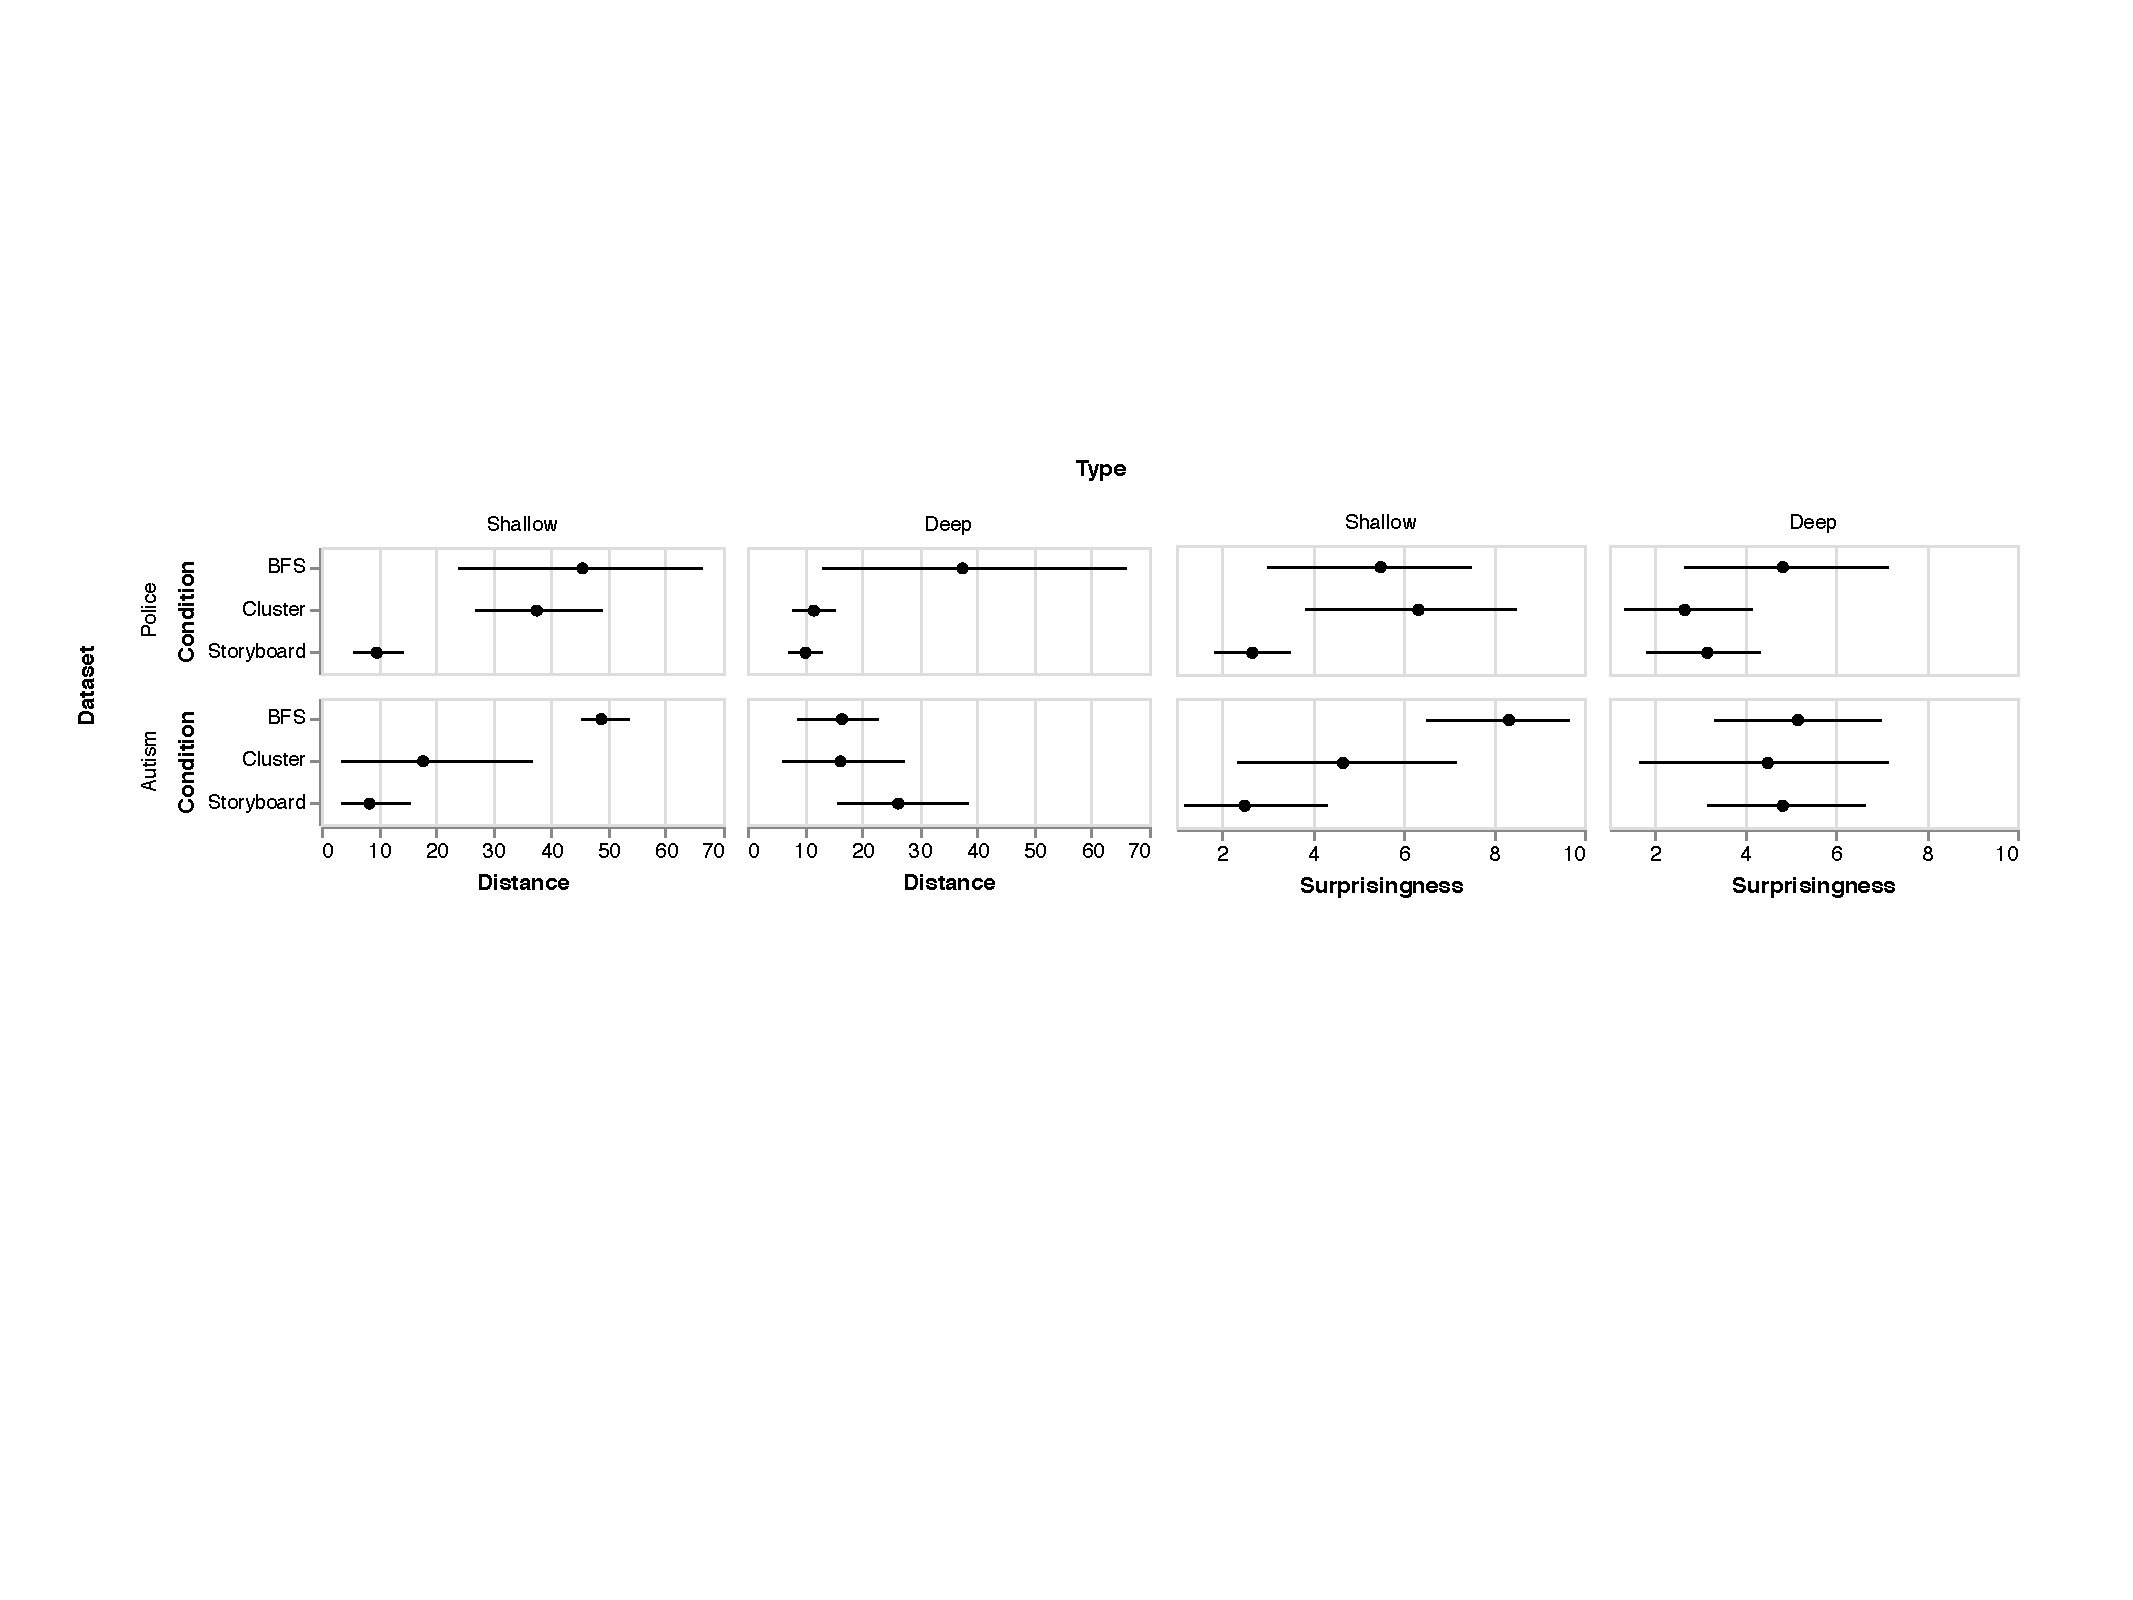
\includegraphics[width=\linewidth]{figures/prediction_results.pdf}
\caption{On the left two columns, Euclidean distance between predicted and ground truth. In general, predictions made using \system is closer to the ground truth. On the right two columns, surprisingness rating reported by users after seeing the actual visualizations on a Likert scale of 10. In general, \system participants had a more accurate mental model of the unseen visualization and therefore reported less surprise than compared to the baseline.}
\label{fig:distance}
\end{figure*}
\stitle{Prediction (RQ3):} Since we can not directly test compare between misleading and informative drill-down paths for RQ3, we use the prediction tasks as a proxy for how informative the selected visualizations in the dashboard are, by measuring how accurate the participants are at predicting an unseen visualization. In order to measure how accurate participants' decisions are, we computed the Euclidean distance between their predicted distributions and ground truth data distributions. As shown in Figure \ref{fig:distance} (top), all the shallow predictions made by using information from the \system\ is closer to the actual distribution compared to the baselines. This aligns with our findings in the formative study and indicates that users are able to more accurately reason about how unseen data would behave with \system. Figure \ref{fig:distance} (bottom) also shows that participants who used \system\ reported that they were less surprised when the unseen visualization is revealed, which again indicates that participants had a more accurate mental model of prediction.
\par \system\ did not perform as well compared to the baselines for the Autism deep prediction task. One possible reason for this is due to the fact that the shallow and deep prediction tasks for the Autism dataset were correlated. Therefore, after learning about the insights that answering 1 on question 9 results in a very high probability for an autism diagnosis, some participants made use of that information when tackling the subsequent deep prediction task. By discussing with the baseline participants on how they have obtained the prediction estimates, they described how surprised they were by the finding in the shallow prediction and therefore adjusted the autism diagnosed values to be higher to compensate for their mistake in the subsequent deep prediction task.
\par We also compute the variance of participants' predictions across the same task. In this case, low variance implies that any user who reads the dashboard is able to provide consistent predictions, whereas high variance implies that the dashboard did not convey a clear data-driven story that could guide their predictions, so instead participants relied on different priors or guessing to form the prediction. These trends can be observed in Figure \ref{fig:actual_predictions}, where the prediction variance amongst participants who used \system\ is much lower than the variance from the baselines.
% \begin{figure*}[bht]
% \centering
% 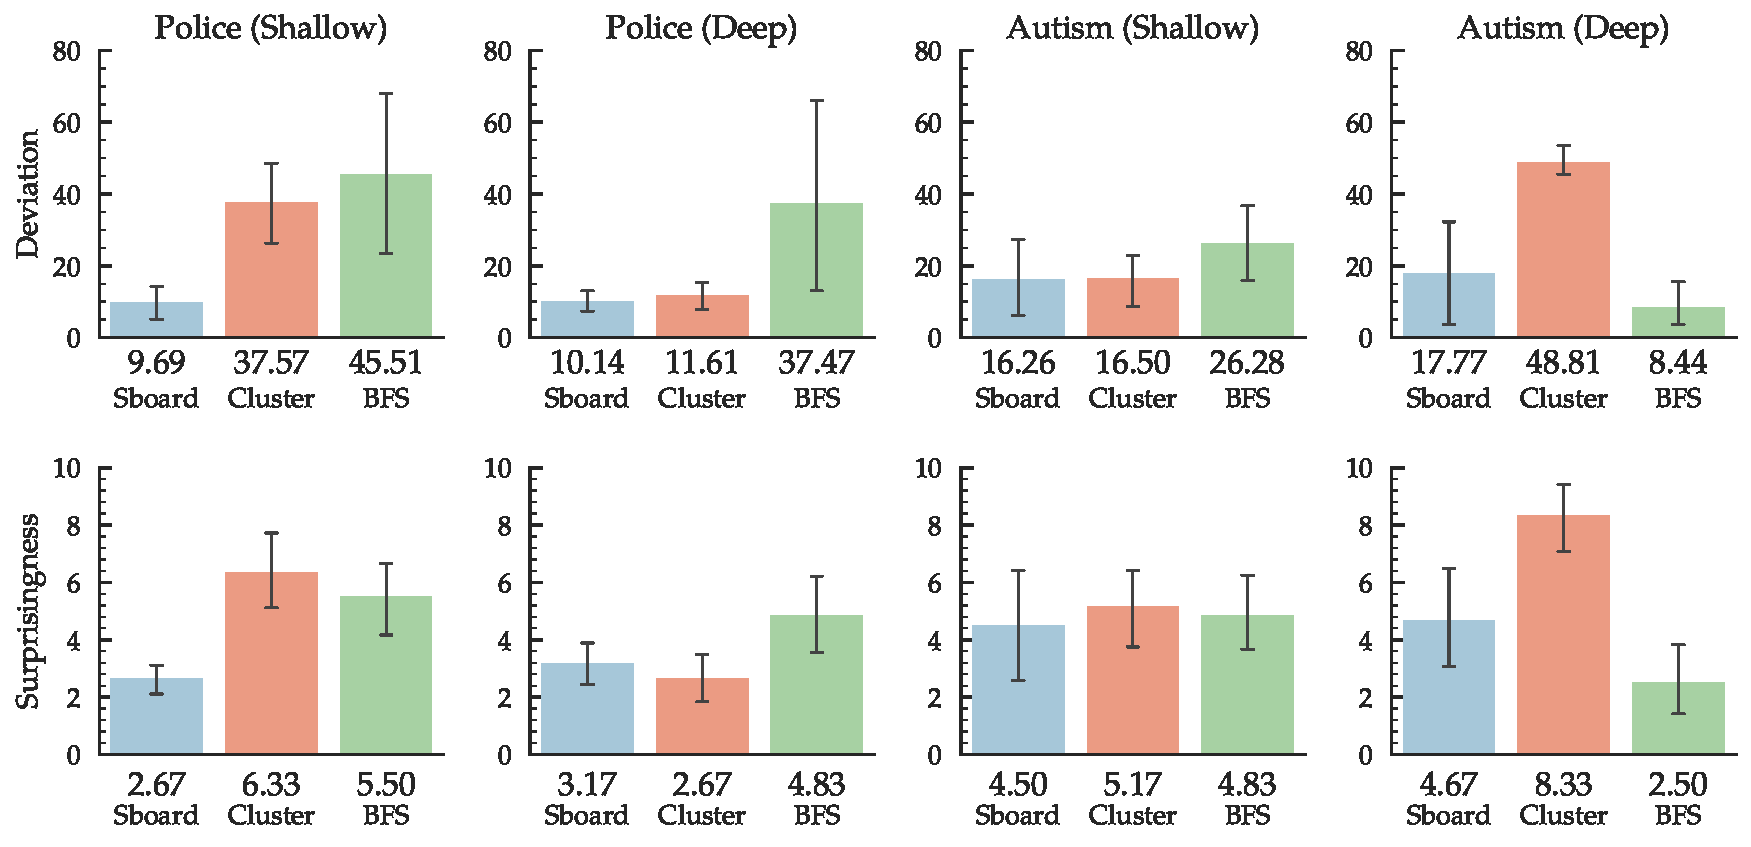
\includegraphics[width=\linewidth]{figures/Devation_Surprisingness.pdf}
% \caption{Top: Euclidean distance between predicted and ground truth. Bottom: Surprisingness rating reported by users after seeing the actual visualizations on a Likert scale of 10.}
% \label{fig:distance}
% \end{figure*}

\begin{figure*}[h!]
\centering
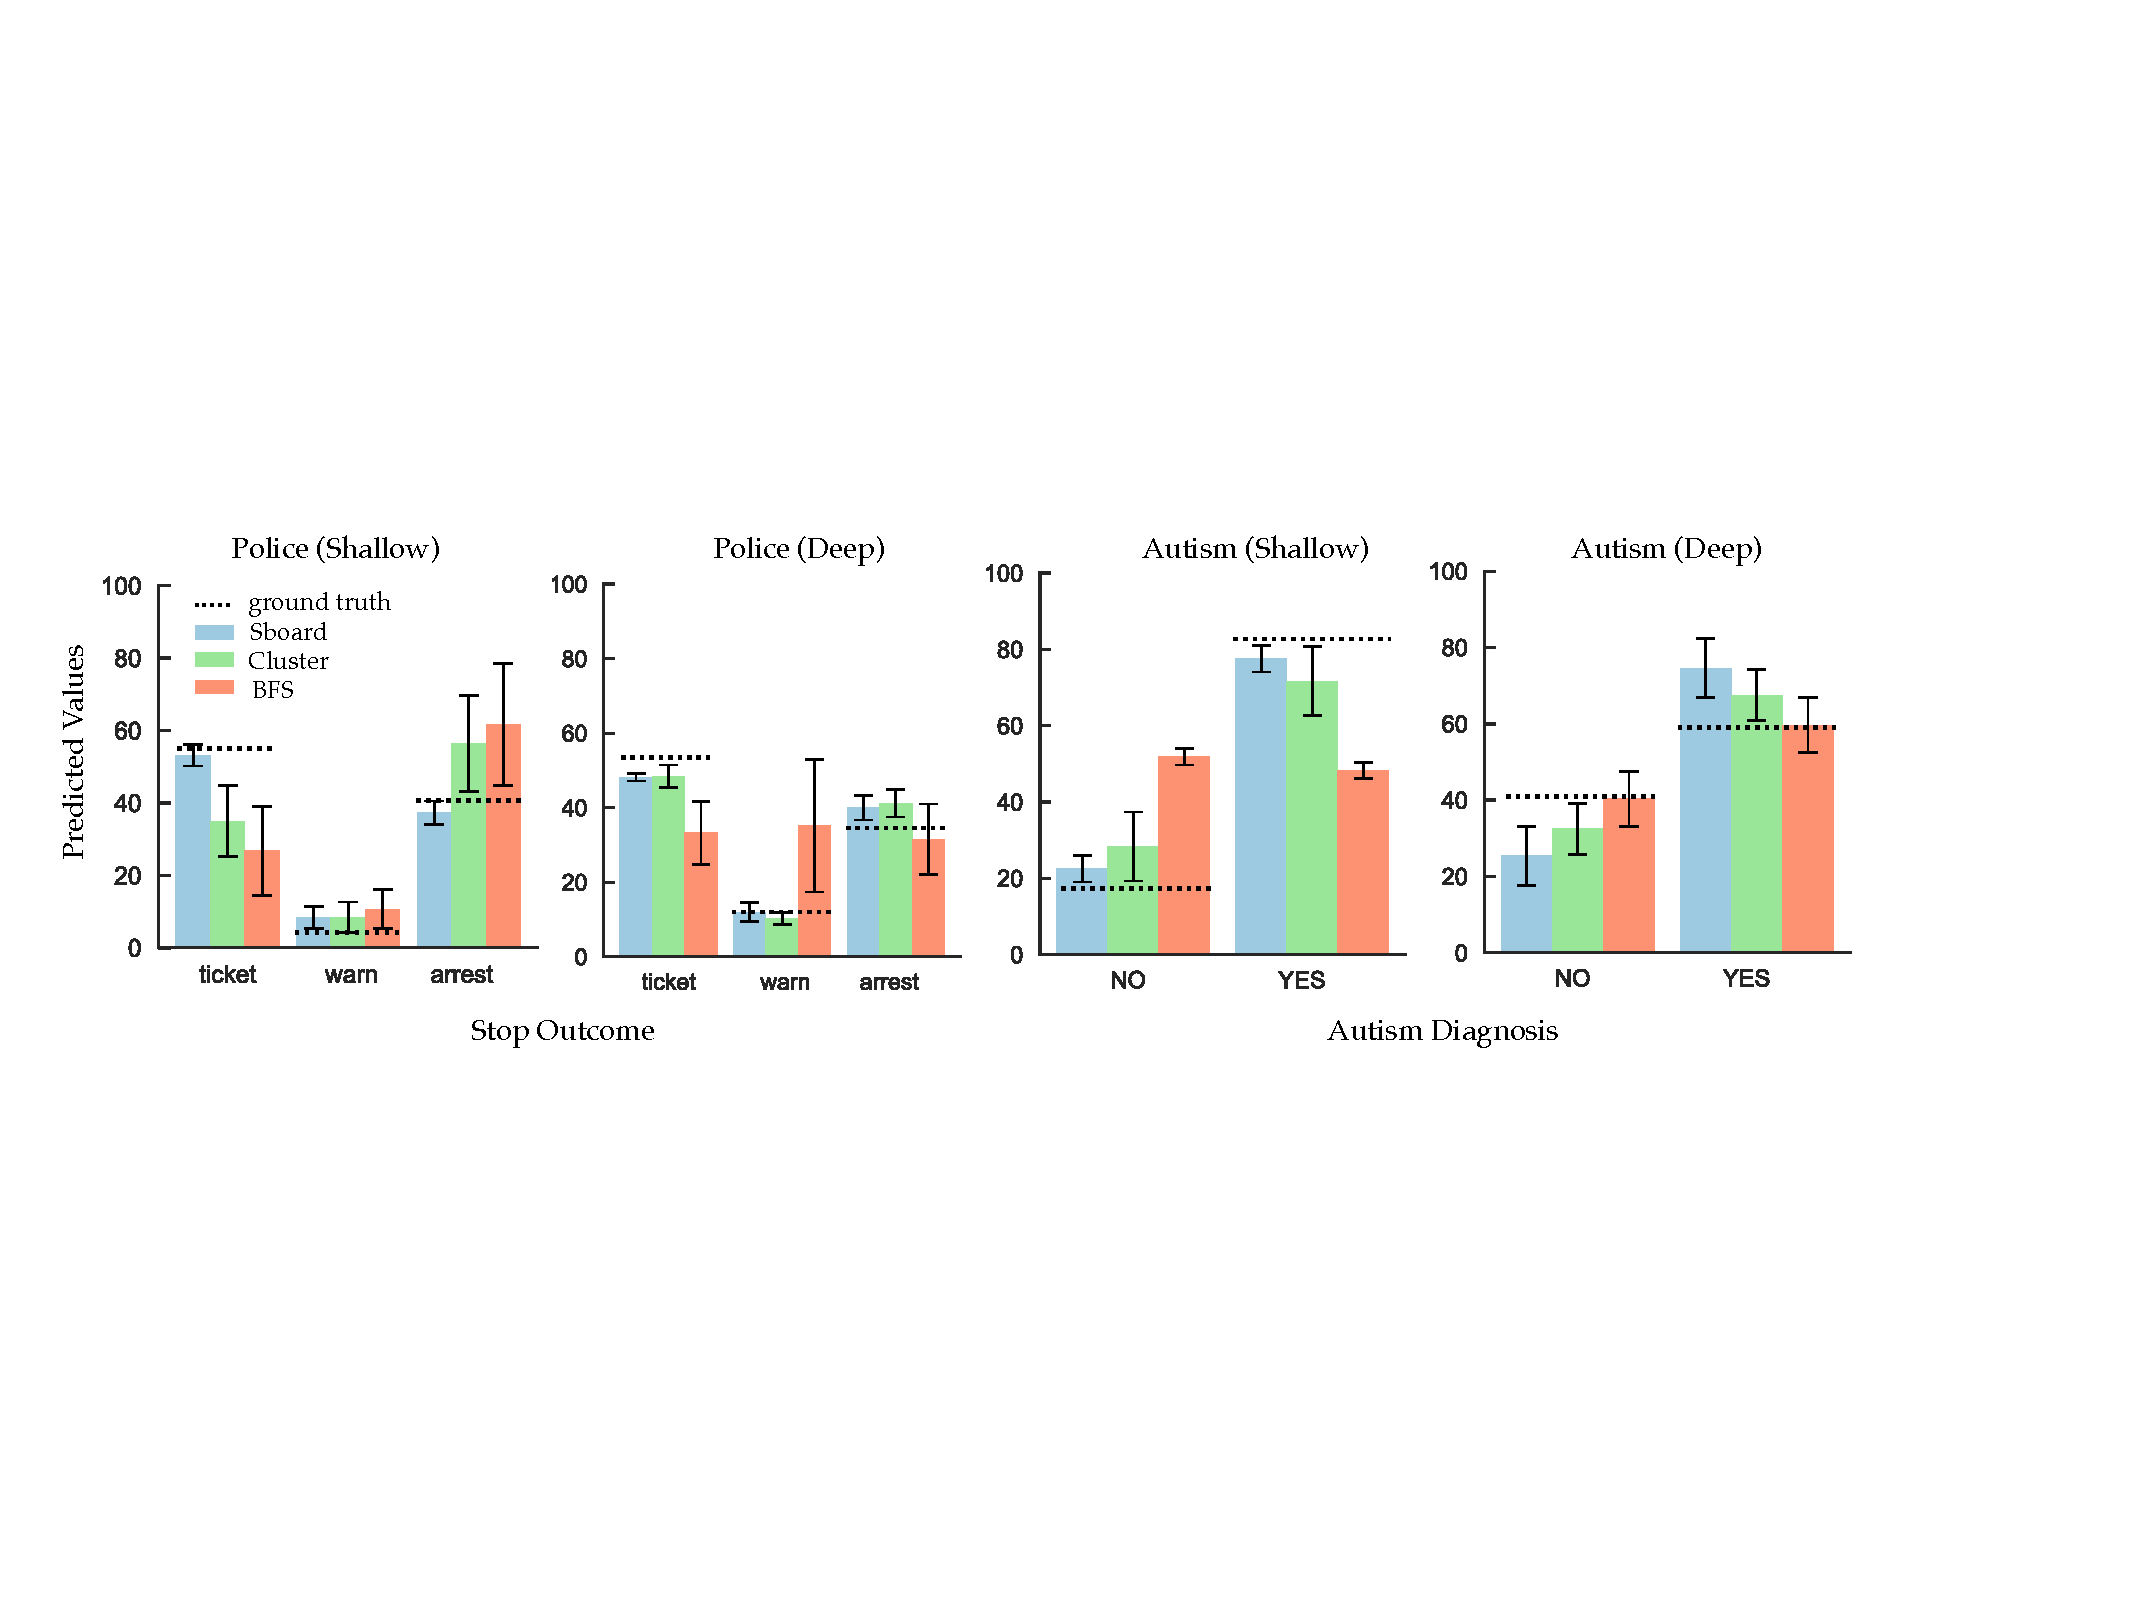
\includegraphics[width=\linewidth]{figures/Prediction_Actual.pdf}
\caption{Mean and variance of predicted values. Predictions based on \system exhibits lower variance (as indicated by the error bars) and great proximity to the ground truth values (dotted).}
\label{fig:actual_predictions}
\end{figure*}

%!TEX root = main.tex
\section{Discussion}
To understand the usefulness of our recommended visualizations, we analyzed the user study transcriptions through an open coding process by two of the authors. For each task in our study, we assigned a binary-valued code to indicate whether or not a participant engaged in that particular task (action or thought process). Table~\ref{table:thematic_summary} highlights results from thematic coding, discussed in this section. We will use the notation [Participant.DatasetAlgorithm] to refer to a participant engaging with a dashboard created by an algorithm=\{1,2,3\}=\{\system, \cluster, \textsc{BFS}\} on a dataset =\{A,B\}=\{Police, Autism\}.
% \stitle{\system promotes distribution-awareness by provoking comparisons against more informative contextual references.}We first studied the thematic codes to understand how participants select contextual references for visualizations. 
\subsection{The Choice of Contextual References}
\par As discussed earlier, analysts often make use of related visualizations as \emph{contextual references}\agp{define if not here, define here.} to form their expectations for unseen visualization. The choices of a proper informative parent is essential for ensuring the \emph{safety} of insights derived through drill-downs. To understand how `safe' the dashboards generated from each condition were, we examined the types of visualizations that participants utilized and compared against to form their expectations regarding how other unseen visualizations should look like. In particular, we thematically encoded participant's use of contextual references based on the verbal explanations that they provided to justify their prediction task responses. Participants can (and often do) make comparisons against more than one type of contextual references to obtain their prediction. We uncovered four main classes of contextual references, described below using the example visualization \texttt{gender=F, race=White, age=21-30} (in the order of most to least similar) and illustrated graphically in Figure~\ref{fig:reference}:
\begin{enumerate}
	\item Parent : Comparison against a visualization with one filter criterion removed (e.g., \texttt{gender=F, race=White})
	\item Siblings : Comparison against a visualization that shares the same parent. In other words, the filter types are the same, but with one criterion changed to inherit a different value. (e.g., \texttt{gender=M, race=White, age=21-30})
	\item Relatives : Comparison against a visualization that shares some common ancestor (excluding overall), but not necessarily the same parent. In other words, these visualizations share at least one common filter type, but with more than one criterion that inherits a different value. (e.g., \texttt{gender=F, race=White, age=60+, search conducted=T})
	\item Overall : Comparison against the distribution that describes the overall population (no filters applied).
\end{enumerate}
\begin{figure}[h!]
\centering
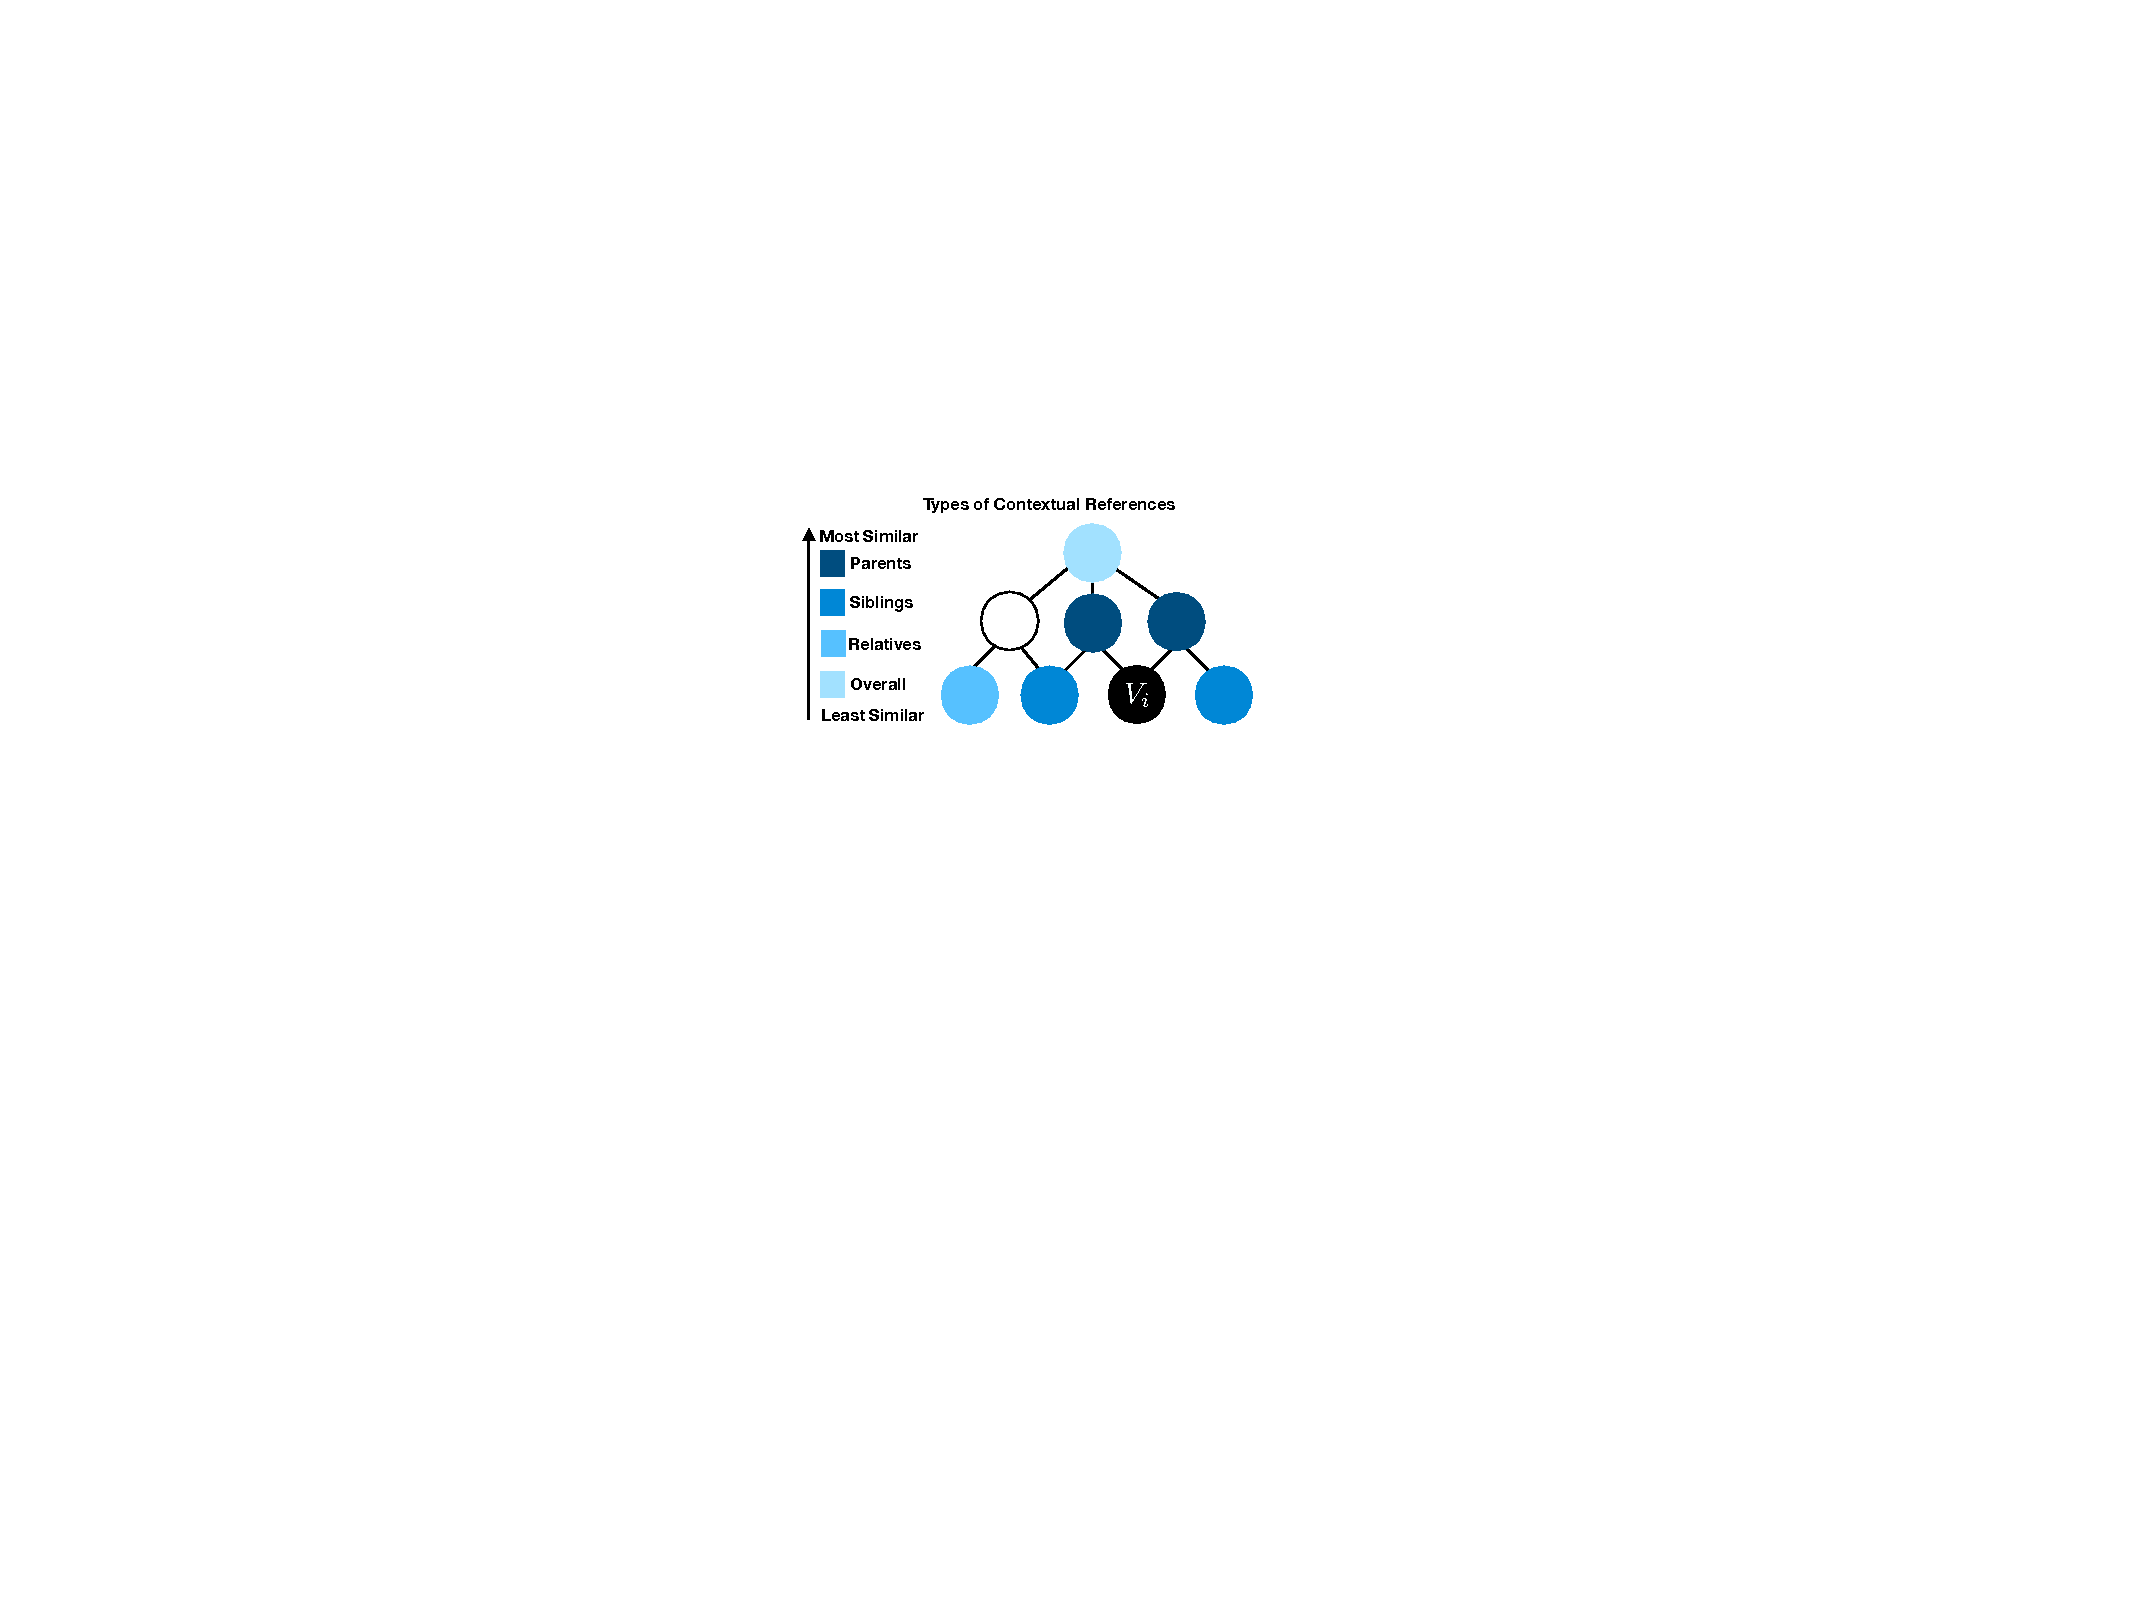
\includegraphics[width=\linewidth]{figures/contextual_reference.pdf}
\caption{Illustrative example of the different types of contextual reference for a given visualization of interest.}
\label{fig:reference}
\end{figure}
As shown in Table \ref{table:contextualReferenceCount}, in general, we find that participants make more comparisons in total using \system than compared to \cluster and \BFS. Studying participants' use of contextual references reveals inherent challenges that arise from using the dashboards generated by \BFS and \cluster. For \cluster , participants mainly compared against relatives and the overall visualizations. Since \cluster optimizes the diversity of shape (distributions) amongst the visualizations, the selected visualizations had up to 4 filters and were disconnected from each other. For this reason, in many cases participants could only rely on relatives and the overall one as contextual references. For example, P4.A2 pointed at a 4-filter visualization with extreme values (100\% for warning; 0\% for arrest and ticket) and indicated how ``\textit{a lot of [the visualizations] are far too specific. This is not very helpful. You can't really hypothesize that all people are going to be warned, because it is such a specific category, it might just be one person}''. %, you need to have a bigger dataset. And that category will not really give you such extremes to make it more credible''.
He further explained how he ``\textit{would not want to see the intersections [(visualizations with many filters)] at first and would want to see all the bases [(univariate summaries)] then dig in from there.}'' The lack of informative contextual references in the \cluster dashboard is also reflected in how analysts exhibited high variance and deviation in their prediction responses.
%despite our modification to KMeans which picks the visualizations with the least number of filters to show in the dashboard for improving interpretability
%These themes are drawn from user's explanations of how they obtained certain insights or ---- that --different tasks or while interpreting the dashboards. 4 categories :
\begin{table}[h!]
\hspace{-10pt}
\centering
	\begin{tabular}{|l|rrrr|r|}
	\hline
	 \small{Algorithm}   &    \small{Parent} &   \small{Sibling} &   \small{Relative} & \small{Overall} &   \small{Total} \\
	\hline
	 \small{\system}     &    \cellcolor{blue!25} 12 &       8 &     0 &  11 &      \cellcolor{blue!25} 31 \\
	 \small{\cluster}     &         4 &        0 &         7 &          8 &      19 \\
	 \small{\BFS}         &         0 &        5 &         1 &          8 &      14 \\
	\hline
	\end{tabular}
\caption{Out of 12 participants, the number of participants who made use of each contextual reference across the two datasets. Participant behavior shows a similar trend in individual datasets. \system participants made more comparisons in general and against parents compared to the baseline.}
\label{table:contextualReferenceCount}
\end{table}
\par For \BFS, most comparisons were based on the overall and siblings. Due to the sequential level-wise picking approach, for the \BFS dashboards, the overall visualization corresponded to the immediate parent, so they are not explicitly recorded as a parent. While the overall and sibling comparisons can be informative, due to the limited number of visualizations ($k$), not all first-level visualizations were displayed in the dashboard. These incomplete comparisons can result in flawed reasoning, as observed in the Autism shallow prediction task described earlier. In contrast, for \system, almost all users compared against the overall and parents, while some also exploited sibling comparison information to make weaker guesses for less-frequently observed attributes (e.g., using a 2-filter sibling visualization involving \texttt{driver\_age} to infer another 2-filter visualization \texttt{driver\_age} with a different parent.)
% \subsection{Improper contextual reference can lead to misleading insights.}
\begin{table*}[ht!]
	\centering
	\begin{tabular}{|l|l|l|l|}
	\hline & \system & \cluster & \BFS \\ \hline
	Difficulty with Interpretating Visualizations & 0 & \cellcolor[HTML]{FD6864}3 & 1 \\ \hline
	Misjudged Significance of Potential Small-Size Population & 0 & \cellcolor[HTML]{FD6864}4 & 1 \\ \hline
	Interpretable ``Human-like" Dashboard & \cellcolor[HTML]{9AFF99}5 & 1 & 0 \\ \hline
	Number of Insights (Police) & \cellcolor[HTML]{9AFF99}11 & 8 & 9 \\ \hline
	Number of Insights (Autism) & \cellcolor[HTML]{9AFF99}16 & 6 & 11 \\\hline
	\end{tabular}
\caption{Summary of qualitative insights from thematic coding. We record the number of insights based on overall findings regarding the dataset or information regarding one or more attributes that are discovered by more than two different participants. There were a total of 7 such insights that we coded for the Police dataset and 6 for the Autism dataset.}
\label{table:thematic_summary}
\end{table*}
\subsection{The Danger of Improper References}
\agp{Can we subdivide each of these up?}
\par While comparisons are essential for data understanding, choosing the wrong contextual reference for comparison could lead to misleading insights. In particular, when a visualization composed of multiple filter conditions is shown in a dashboard created using \cluster, 25\% of participants had trouble interpreting the meaning of the filter for at least one of the datasets. In contrast, as shown in Table~\ref{table:thematic_summary}, this confusion only happened once for \BFS and none for \system. This is due to the fact that \cluster dashboards are seemingly random to the users, whereas \BFS and \system both have a more natural, interpretable ordering. In addition, when examining visualizations with many filters along with extremely-skewed values in one or more bars (bars with 100\% or 0\%), 4 \cluster participants did not realize that charts with multiple filters may have a smaller subpopulation size, echoing our previous concern regarding the danger of small subpopulation sizes. This issue stems from the fact that the contextual reference used for comparison was the overall population, however the unseen parent subpopulation may have behaved very differently. This subpopulation-size fallacy was observed to be more severe for the Autism dataset, where participants had less intuition on the expected attribute behavior. In contrast, 6 of the participants using \system explicitly noted that while these extreme-valued visualizations may be interesting, they were less certain due to the unknown subpopulation size and should be investigated further. For example, P1.A1 noted that a visualization with warning=100\% caught her eye, ``\textit{but I don't know what the N is, maybe it's one person, this makes me a little skeptical, that makes me want to go back to the raw data and look at what is the N and what drives something so drastic?}'' Since \BFS dashboards only displayed first-level visualizations, participants for \BFS did not see such visualizations during the study session, so none of the \BFS participants exhibited signs of this fallacy.

% \subsection{Hierarchical layout leads to more natural contextual comparisons compared to table layout.}
\subsection{Interpretability of Hierarchical Layouts}
\par In the post-study interviews,  participants cited hierarchical layout as one of the key reasons why it was easier to follow contextual references in \system. Users were able to easily interpret the meaning of the dashboard through \system's hierarchical layout, even though they were never explicitly told what the edge connections between the visualizations meant. For example, P1.A1 stated that ``\textit{the hierarchical nature [is] a very natural flow...so when you are comparing, you don't have to be making those comparisons in your head, visually that is very pleasing and easy to follow.}'' %Likewise, [P8.A1] also stated that ``I like the different levels, it makes it very visually easy to figure out what you want to look at, if you want to look at the overall data, it's right there at the top for you, if you want to get more specific, you just follow a branch downwards, which I think is very intuitive.''
Likewise, P9 described how the hierarchical layout she saw for the Autism dataset was a lot easier to follow than the Police dataset shown in the table layout for \cluster:
\begin{quote}
\textit{If I had to look at this dataset in the format of the other one, this would be much more difficult. It was pretty hard for me to tell in the other one how to organize the tree, if there was even a tree to be organized. I like this layout much better, I think this layout allows me to approach it in a more meaningful way. I can decide, what do I think matters more: the overall trend? or the super detailed trends? and I know where to look to start, in the other one, every time I go back to it, I would say, where's the top level, where's the second level? I mentally did this. Like when you asked me that first question, it took much longer to find it, because I literally have to put every chart in a space in my head and that took a lot longer than knowing how to look at it.}
\end{quote}
At the end of the study, some participants who saw table layouts sketched and explained how they would like the layout of the visualizations to be done. Participants expressed that they wanted ``groupings'' or layouts that arranged visualizations with the same attribute together. Other participants advocated for isolating the overall visualization outside of the dashboard table for facilitating easier comparisons. Both of these provides further motivation for our hierarchical layout and the idea of the collapsed visualizations as described in the System section.%in Section \ref{sec:interaction}.
\par Since we did not inform participants about how the dashboards were generated, it was also interesting to note that some participants thought that the dashboards were hand-picked by a human analyst and described what this person's intentions were (e.g., ``\textit{It seems like the researcher who created this dashboard was specifically looking at people of Asian descent and people who are 60 or older.}'' [P7.A1]). We encoded this phenomenon by looking at instances where a participant either explicitly referring to a person who picked out the dashboard or implicitly described their intentions through personal pronouns. As summarized in Table~\ref{table:thematic_summary}, a total of 5 different participants referred to the \system dashboards as if they were generated by a human, whereas there was only 1 participant for \cluster and none for \BFS made such remarks. At the end of the study, many were surprised to learn that the \system dashboard was actually picked out by an algorithm, indicating that \system could automatically generate convincing dashboard stories similar to a dashboard that was authored with human intention.
\stitle{Limitations of \system}
% Interestingness task is highly subjective, so not conclusive whether interesting or not , despite the positive result
% Due to the highly subjective nature of the retrieval task, the interestingness selection for the Police dataset was biased by participant's priors and intuition about the attributes. For example, while all participants who have seen the visualization "duration=30+min" verbally noted that stop duration is a crucial factor that leads to arrest, only 4 users marked it as interesting. 5 participants marked the visualization as not interesting and 4 left it unselected, because the visualization was not very surprising as it agreed with their intuition that ``\textit{if the police stop is taking a long time, something has probably gone wrong}''.
\par As described earlier, since the details of how the dashboard was obtained was not explained to the users during the study, some users expressed that they were initially confused by \system since not all variables were present in the dashboard. Others also found it confusing that the addition of filters did not always correspond to the same variables. For example, P2.A1 criticized how the dashboard was intentionally selected to be biased:
\begin{quote}
\textit{I feel like this one, not all the data is here, so we are already telling a story, you are trying to steer the viewer to look at certain things. And the focus seems to be on where the arrest rate is high. You probably could have found other things that led to ticket being high, but you didn't pull those out. You are trying to see if there are other factors that leads to more arrests.}
\end{quote}
\npar This sentiment is related to participants' desire to perform their own ad-hoc querying alongside the dashboard to inspect other related visualizations for verifying their hypothesis. For example, P7.A1 wanted to inspect all other first-level visualizations for driver's race to assess its influence. P7.A1 expressed that while he had learned many insights from the dashboard, ``\textit{the only thing I don't like is I cannot control the types of filter, which is fixed.}'' Outside the context of the user study, it is essential to explain how \system are picking the visualizations in a easy and interpretable manner to establish a sense of summarization guarantee for the users and help them make better inferences with the dashboard.
\par As discussed earlier, the subpopulation size is important in establishing the significance of a trend observed in a visualization. While subpopulation size is taken into account implicitly in our objective, we should design interfaces that can convey the notion of subpopulation size in our dashboard. Examples include Sankey-like flow diagrams indicating the percentage of the parent population broken down into individual subpopulations or subpopulation size explicitly specified via edge labels.%, either explicitly displayed as text when hovering over the visualization or changing the size or background color of the visualizations to encode subpopulation size.
%“I actually found it really confused at first because such a low arrest rate at the top, and then at the bottom the arrest rate was much higher, so I was like is this data wrong. Then I realized we’re not looking at all the data here, you’ve pulled out some of it. It took me a minute to realize that. And once I read the title of the charts I realized that makes sense.” [P2.A1]
% - Reference of Comparison
% - Layout naturally lends itself for comparison:
% 	- describe ordering layout, how participants naturally follow the flow
% 	- emph that we did not tell them what the edge connections mean and how they were computed but the users naturally figured it out, that it means adding an additional filter.
% 	- hierarchical interpretable nature (quotes)
% 	- compared to other baselines
% 	- describe dashboard by human (count)
% - Misleading insights v.s. True insight discovery rates
% 	- Interpretability:
% 	- misled understanding subpopulation size
% 		- for autism, it is important to see if they compare to overall because if not they would think high skew to NO is important whereas its actually pretty close to overall.
% 	- trouble interpreting filter combination
%%%%%%%%%%%%%%%%%%%%%%%%%%%%%%%%%%%%%%%%%%%%%%%%%%%%%%%%%%%%%%%%%%%%%%%%%%%%%%%%%%%%%%%%%%%%%%%%%%%%%%%%%%%%%%%%%%%%%%%%
%%%%%%%%%%%%%%%%%%%%%%%%%%%%%%%%%%%%%%%%%%%%%%%%%%%%%%%%%%%%%%%%%%%%%%%%%%%%%%%%%%%%%%%%%%%%%%%%%%%%%%%%%%%%%%%%%%%%%%%%
%%%%%%%%%%%%%%%%%%%%%%%%%%%%%%%%%%%%%%%%%%%%%%%%%%%%%%%%%%%%%%%%%%%%%%%%%%%%%%%%%%%%%%%%%%%%%%%%%%%%%%%%%%%%%%%%%%%%%%%%
% \subsection{Statistical Paradoxes}\dor{make title full sentences}
% Visualizations are powerful representations for studying different distributions or patterns in a dataset, but our human intuition could often mislead us when it comes to interpreting those patterns\cite{Binnig2017,Wall2017}. Several statistical paradoxes can lead analysts to draw incorrect conclusions from observed visualizations, including Simpson's paradox as discussed in the introduction. The key reason why many of these paradoxes emerge is the \emph{incompleteness} of the observed data or lack of focus on relevant informative subsets of the data. For example, Simpson's paradox arises in the presence of an unseen confounding variable. %likewise, the absence of  base rate information causes base rate fallacy.
%  We assert \dor{too strong of a sentence} that distributional awareness can be useful in avoiding such statistical paradoxes. If an analyst is aware of all distributions in a given dataset, he/she is less prone to many statistical paradoxes. However, given the large number of dimensions and high cardinality of these dimension in modern datasets, it is not possible for an analyst to explore and memorize all distributions. Therefore, a more evolved approach is to be aware of the exceptional distributions. In this work, we propose a first step towards this goal, where we identify the exceptional distributions in terms of their informative references. The remaining (unseen) distributions in the dataset are rather unsurprising and can be inferred from the visualizations in the dashboard. \dor{I would recommend first talk about issue with large dimension + danger of multiple hypothesis testing + incomplete testing, point out problem, then talk about how our system resolves this.}
% \subsection{Structural Insight}
% Our proposed dashboard consists of a hierarchy of visualizations, where each visualization is linked to its most informative parent. The shape or structure of the hierarchy contains useful information that augments the information learned from the visualizations and aid distribution awareness and understanding. \dor{what's interesting here is that while many work have looked at visualization presentation, layout of presentation never considered, we find in Sec 5 that this is actually important and can encode info.} For example, the depth and branching factor of the hierarchy could inform a user regarding the configuration of insights. Deep hierarchies contain long paths, i.e., insights are present at lower level visualizations with multiple constraints. In contrast, bushy hierarchies (with high branching factor) contain cases where multiple visualizations have the same informative parent and they differ from that parent. \dor{do we have examples from the study that support this?} We assert that the depth and branching factor could be a meaningful constraint in our problem formulation \dor{too strong of a sentence}. Some applications for example, funnel exploration require studying deep hierarchies, whereas others for example, building decision trees require studying bushy hierarchies. A natural extension of our current problem formulation is to allow users to select the depth and branching factor for the hierarchy. 
% \subsection{Other Visualization Lattices}
% In this work, we explore the space of data subsets to generate our visualization lattice. Note that it is possible to explore the space of dimension attributes in x-axis to generate a different visualization lattice. In particular, given a combination of dimension attributes $X = \{X_1, \ldots, X_n\}$, adding one or more new dimensions in $X$ will generate a new combination. An ancestor-descendant relationship exists between these dimension combinations, following the same principles of Section 3.1. These relationships lead to a new lattice, which we call the dimension combination lattice. Our informative deviation based approach could be used for traversing the dimension combination lattice. However, we observe that most users do not visualize more than two attributes in x-axis. Therefore, traversing the dimension combination lattice is not very useful for most applications.
% \dor{I think 6.2,6.3 don't tie well with the rest of the paper. It sounds like stretching our own ideas rather than being motivated by the work done in this paper. Other potentially more relevant discussion: distribution awareness and how it might be useful in other contexts? Decision trees?}
% %\subsection{Utility Metrics} 
%!TEX root = main.tex
\section{Related Work}
Our work draws from, and improves upon, several research threads.

\subsection{Guided Exploration of Multidimensional Data}
Given a dataset, tools such as Spotfire and Tableau supports automatic selection of visualizations (e.g., Show Me~\cite{Mackinlay2007} by Tableau) based on aesthetics. There's a more recent body of work that automatically selects visualizations based on statistical measures such as scagnostics and deviation. Given a scatterplot, Anand et al. \cite{Anand2015} uses randomized permutation tests to select partitioning variables that reveals interesting small multiples based on scagnostics. Given an input bar chart, Vartak et al. \cite{Vartak2015} finds interesting bar charts that deviate form the input chart using a deviation-based measure. Our work extends the deviation-based measure to formulate user's expectation. However, unlike the existing systems, we concentrate on informativeness, which enables our systems to prevent the drill-down fallacy.
%\cite{Elmqvist2008Rolling} presents an interactive tool to explore multidimensional data using a matrix of scatterplots that shows the relationship between all pairs of attributes.

\subsection{Preventing Biases and Statistical Fallacies}
Visualizations are powerful representations for studying patterns in a dataset, but our human intuition could mislead us when it comes to interpreting those patterns~\cite{Wall2017, Alipourfard2018WSDM, Zgraggen2018CHI}. Wall et al.~\cite{Wall2017} presents six metrics to systematically detect and quantify bias from user interactions in visual analytic systems. These metrics are based on the concepts of coverage and distribution, focusing on the assessment of the process by which users sample the data space. Alipourfard et al.~\cite{Alipourfard2018WSDM} presents a statistical method to automatically identify Simpson’s paradox by comparing statistical trends in the aggregate data to those in the disaggregated subgroups. Zgraggen et al.~\cite{Zgraggen2018CHI} presents a method to detect Multiple Comparisons Problem (MCP) in visual analysis. In this paper, we concentrate on drill-down fallacy, a fallacy that has not been addressed before in visual analytics literature.

\subsection{Storytelling with Visualization Sequences}
Visualizations are often arranged in a sequence to narrate a data story. Existing work on visualization sequences and storytelling have studied the structures of narrative visualizations\cite{Segel2010,Hullman2017}, effects of augmenting exploratory information visualizations with narration\cite{Boy2015} and, more recently, ways to automate the creation of visualization sequences\cite{Hullman2013,Kim2017}. Most of these work have adopted a linear layout (motivated by slidedecks) to present the visualization sequences. Hullman et al. \cite{Hullman2017} found that most people prefer visualization sequences structured hierarchically based on shared data properties such as levels of aggregation. Kim et al. \cite{Kim2017} models relationships between charts by empirically estimating transition (edge) cost between moving from one visualization (node) to another. They find that participants preferred ``\textit{starting from the entire data and introducing increasing levels of summarization}''. Our work is the first to automatically organize visualizations in a hierarchical layout for summarizing the space of data subsets.

%Both \cite{Hullman2013,Kim2017} use a graph model to formalize the visualization design space.
%In addition, we present a novel problem formulation that recommends a connected visualization sequence in a hierarchical layout summarizing the space of data subsets.

\iffalse
\section{Related Works}
\npar \stitle{Storytelling with visualization sequences:}
Visualizations are often arranged in sequence to narrate a data story. Existing work on visualization sequences and storytelling have studied the structures of narrative visualizations\cite{Segel2010,Hullman2017}, effects of augmenting exploratory information visualizations with narration\cite{Boy2015} and, more recently, ways to automate the creation of visualization sequences\cite{Hullman2013,Kim2017}. Most of these work have adopted a linear layout (motivated by slidedecks) to present the visualization sequences. Hullman et al. \cite{Hullman2017} found that most people prefer visualization sequences structured hierarchically based on shared data properties such as levels of aggregation. %Both \cite{Hullman2013,Kim2017} use a graph model to formalize the visualization design space.
Kim et al. \cite{Kim2017} models relationships between charts by empirically estimating transition (edge) cost between moving from one visualization (node) to another. They find that participants preferred ``\textit{starting from the entire data and introducing increasing levels of summarization}''. Our work is the first to automatically sequence visualizations in a hierarchical layout for summarizing the space of data subsets. %In addition, we present a novel problem formulation that recommends a connected visualization sequence in a hierarchical layout summarizing the space of data subsets.

\subsection{Visualization recommendation}
\par%Despite the large body of work that recommends informative visualizations given pre-selected data attributes and aggregations, the data selection problem is a more important problem in exploratory data analysis, since the analysts have to figure out which groups of data attributes would be of interest in order avoid manual exploration of the data.
Visualization recommendation systems select appropriate visualizations to show based on an objective function. The metrics considered by these systems can largely be divided into two categories: perceptual or data-driven. The first type of recommendation system selects visualizations based on its visual effectiveness and expressiveness~\cite{Wongsuphasawat2016,Mackinlay2007}. Our work is more related to the latter category of systems which uses statistical measures computed based on the underlying data subset, such as cognostics or deviation. Anand et al. \cite{Anand2015} used randomized permutation tests to automatically select partitioning variables to display visualizations exhibiting patterns that are different from the input visualization as determined by its cognostic score. Vartak et al. \cite{Vartak2015} finds interesting visualizations by a deviation-based measure between the user's query view and reference view, given a query of interest. While both existing systems require the analyst to input a visualization of interest as a query, our paper extends the deviation-based idea to establish user's expectation using informative parent enabling \system to traverse the visualization lattice in search of a connected, maximally informative and interesting story without the need for an input query.  %Wongsuphasawat et al. \cite{Wongsuphasawat2016} presents a mixed-initiative system where the users direct the variables of interest and the system suggests other variables that may be potentially interesting to the user. Since this is a mixed-initiative system rather than an automatic recommendation engine, the system only ``looks ahead" one variable at a time. Their goal is to promote breadth-oriented data exploration rather than helping users find interesting stories or visualizations.

%- the issue of surprisingness metric and ---- have been examined before for viz, but none have looked at data subset lattice specifically for viz

\subsection{Data Exploration of OLAP Data Cubes} %\dor{This may be a bit long and need to be cut, I didn't include related works on surprisingness metrics (e.g. Bayesian Cognition paper, Surprise Map ,etc.). Can add if necessary.}
The challenge of manual, unguided search in online analytical processing (OLAP) applications have been well studied in the context of data cube exploration by Sarawagi et al. ~\cite{Sarawagi1999,Sarawagi2000,Sarawagi1998}. To address this challenge, they simplify the search by identifying ``interesting'' regions of a data cube. These techniques includes precomputed statistics accounting for the surprisingness attributed to neighboring paths to cell and amount of deviation from constrained maximum entropy-based expectations. While these interesting sub-cubes correspond to finding filter combinations for constructing the aggregate visualization in \system, our lattice search space enforces fixed x, y and aggregation as well as connectedness during traversal to discover more interpretable stories.

%Sarawagi et al.\cite{Sarawagi1998} introduced the problem that manual, unguided search for seeking interesting patterns in a datacube is inefficient and requires large numbers of online analytical processing (OLAP) operations, such as roll-up, drill-down, slicing, and dicing. They proposed a discovery-driven approach to data exploration to simplify the search for \textit{exceptions} in the data, based on precomputed statistics regarding how surprising a data cube cell is, relative to neighboring cells at the same level of aggregation, at levels of aggregation below the cell, and along the drill-down path. Sarawagi \cite{Sarawagi1999} presents an OLAP operator that summarizes the reasons for variation in a data view, by computing the information theoretic distance between the immediate parent and its child nodes.
% \par While Sarawagi et al. \cite{Sarawagi1998} takes a more data-driven approach of finding exceptions intrinsic to a given datacube, Sarawagi \cite{Sarawagi2000} envisions a more user-centric application where the comparisons are based only on parents of seen visualization. The user's expectation regarding an unseen visualization is based on the maximum entropy principle where the relationships between the attributes should be maximally uniform across all dimensions, while being consistent with constraints from seen visualizations. The visualization that deviates the most from the user expectation is regarded as an ``interesting" visualization. They take an iterative approach to find the unique solution for the expected values for each attribute from the constrained maximum entropy problem and employ several optimization strategies (reusing computed values, sharing storage of contiguous regions, pruning constraints that subsumes one another or with little influence). Our coverage-based models improve on the iterative approach in providing a tighter constraint to the variable regions of the bars.
\fi

%!TEX root = main.tex
\section{Conclusion}
\par Common analytics tasks, such as causal inference, feature selection, and outlier detection require studying data distributions at different levels of data granularity~\cite{Anand2015,Wu2013,Heer2012}. However, without knowing \textit{what} subset of data contains an insightful distribution, manually exploring distributions from all possible data subsets can be tedious and inefficient. Moreover, when examining data subsets by adding one filter at a time, analysts can fall prey to the drill-down fallacy, where they mistakenly attribute the interestingness of a visualization to a ``local difference'', while overlooking a more general explanation for the root cause of the behavior. To address these issues, we presented \system, an interactive visualization recommendation system that automatically selects a small set of informative and interesting visualizations to summarize the distributions within a dataset. Our user study results demonstrate that our tool can guide analysts towards more informed decisions for retrieving interesting visualizations, judging the relative importance of attributes, and predicting unseen visualizations, than compared to the two other summarization baselines. Study participants also find dashboard generated by \system to be more interpretable and ``human-like'', leading to more discovered insights. Our work is one of the first automated systems that guides analysts across the space of data subsets by summarizing key insights with safety guarantees---a step towards our grander vision of developing intelligent tools for accelerating and assisting with visual data discovery.  
% discovery 
% - Drill down is hard and dangerous
% - Drill down fallacy
% - In this paper, we develop ----
% - \system does X, Y , Z
% Our user study shows that ----\system compared to baselines
% 	- perform better in a wide range of analytic task such as attribute ranking, prediction, and interestingness. 
% 	- interpretable, more insights
% - Wider implications
\bibliographystyle{SIGCHI-Reference-Format}
% \bibliographystyle{ACM-Reference-Format}
\bibliography{reference}

\end{document}
